\documentclass{dissert}
\usepackage{cmap}
\usepackage[T2A]{fontenc}
\usepackage[utf8]{inputenc}

%\usepackage[cp1251]{inputenc}
\renewcommand{\rmdefault}{cmr}
\usepackage{dsfont} % for indicator function
\usepackage[russian]{babel}

\usepackage{color}
\usepackage{caption}
\usepackage{float}
%\usepackage{slashbox}
%пакеты и команды, необходимость в которых может возникнуть по ходу работы (Вы можете добавлять свои):
\usepackage{indentfirst}%для отступов
%\usepackage{subfig}

\usepackage{geometry}
\geometry{left=2.5cm}
\geometry{right=1.0cm}
\geometry{top=2.0cm}
\geometry{bottom=2.0cm}
\renewcommand{\baselinestretch}{1.0}

%\usepackage[backend=biber,style=alphabetic]{biblatex}    

%\usepackage{geometry}
%\emergencystretch=25pt%для борьбы с переполнениями за счет разреж. слов в абзаце
%\righthyphenmin=2% для разрешения переноса двух последних букв
%\arrayrulewidth=.75pt% регулируем толщину линий в табл.
%\usepackage[dvips]{graphicx}%для включения PS файлов
%\usepackage[final]{epsfig}
\usepackage{multicol}%для организации многоколоночного текста (предм. указатель)
\usepackage{subfigure}
\usepackage{indentfirst}
\usepackage{amsmath}
%\usepackage{enumerate}
\usepackage{amssymb}
\usepackage{amsthm}
\usepackage{amscd}
\usepackage{hhline}
%\usepackage{multirow}
\usepackage{graphicx, epsfig}
%\usepackage{epic}
\usepackage{amscd}
%\usepackage{ecltree}
\usepackage{color}
\usepackage[dvips,all]{xy}
%\usepackage{setspace}
%\usepackage{makeidx}
%пакет для вкл символов напр номер
%\usepackage{textcomp}
%\usepackage{amsfonts}
%\usepackage{afterpage}% Полезно для полного заполнения страниц перед большими таблицами
%\usepackage{longtable}%Для таблиц на нескольких страницах
%\usepackage{cite}
%\usepackage{rawfonts}
%\usepackage{oldlfont}%доступ к шрифтам через устаревшие команды
\usepackage{array}
%\renewcommand{\bibname}{Список литературы}
\renewcommand{\contentsname}{Содержание}
\renewcommand{\contentsdesc}{Стр.}
\renewcommand{\chaptername}{Глава}


%%% Библиография %%%
\makeatletter
\bibliographystyle{utf8gost71u}     % Оформляем библиографию по ГОСТ 7.1 (ГОСТ Р 7.0.11-2011, 5.6.7)
%\renewcommand{\@biblabel}[1]{#1.}   % Заменяем библиографию с квадратных скобок на точку
\makeatother

%\def\BibUrl#1.{}
%\bibliographystyle{gost2008} 
\theoremstyle{definition}
\newtheorem{theorem}{Теорема}
\newtheorem{lemm}{Лемма}
\newtheorem{defin}{Определение}
\newtheorem{utv}{Утверждение}

\def\bbljan{Январь}
\def\bblfeb{Февраль}
\def\bblmar{Март}
\def\bblapr{Апрель}
\def\bblmay{Май}
\def\bbljun{Июнь}
\def\bbljul{Июль}
\def\bblaug{Август}
\def\bblsep{Сентябрь}
\def\bbloct{Октябрь}
\def\bblnov{Ноябрь}
\def\bbldec{Декабрь}


\renewcommand{\thesubfigure}{\asbuk{subfigure}}

\graphicspath{{pic/}}


% opers
\DeclareMathOperator*{\indicator}{\mathds{1}}
\DeclareMathOperator*{\softmax}{softmax}
\DeclareMathOperator*{\idx}{idx}
\DeclareMathOperator*{\pos}{pos}
\DeclareMathOperator*{\AUCH}{AUCH}
\DeclareMathOperator*{\tf}{tf}
\DeclareMathOperator*{\ntf}{ntf}
\DeclareMathOperator*{\idf}{idf}
\DeclareMathOperator*{\ndf}{ndf}
\DeclareMathOperator*{\similarity}{sim}
\DeclareMathOperator*{\argmin}{arg\,min}
\DeclareMathOperator*{\const}{const}
\DeclareMathOperator*{\dBeta}{Beta}
\DeclareMathOperator*{\dDir}{Dir}
\DeclareMathOperator*{\Tr}{Tr}
\DeclareMathOperator*{\dDP}{DP}
\DeclareMathOperator*{\dMult}{Mult}
\DeclareMathOperator*{\dBern}{Bern}
\DeclareMathOperator*{\dCRP}{CRP}
\DeclareMathOperator*{\dKL}{KL}
\DeclareMathOperator*{\diag}{diag}
\newcommand{\dd}[1]{\mathrm{d}{#1}}

% BOLD
\newcommand{\bmatr}{{\mathbf{B}}}
\newcommand{\cmatr}{{\mathbf{C}}}
\newcommand{\hmatr}{{\mathbf{H}}}
\newcommand{\fmatr}{{\mathbf{F}}}
\newcommand{\mmatr}{{\mathbf{M}}}
\newcommand{\xmatr}{{\mathbf{X}}}
\newcommand{\pmatr}{{\mathbf{P}}}
\newcommand{\xmatrt}{{\tilde{\mathbf{X}}}}
\newcommand{\imatr}{{\mathbf{I}}}
\newcommand{\vmatr}{{\mathbf{V}}}
\newcommand{\wmatr}{{\mathbf{W}}}
\newcommand{\umatr}{{\mathbf{U}}}
\newcommand{\zmatr}{{\mathbf{Z}}}
\newcommand{\zmatrt}{{\tilde{\mathbf{Z}}}}
\newcommand{\Tmatr}{\mathbf{T}}
\newcommand{\lambdamatr}{{\mathbf{\Lambda}}}
\newcommand{\phimatr}{\mathbf{\Phi}}
\newcommand{\sigmamatr}{\mathbf{\Sigma}}
\newcommand{\thetamatr}{\boldsymbol{\Theta}}

\newcommand{\ab}{{\mathbf{a}}}
\newcommand{\bb}{{\mathbf{b}}}
\newcommand{\cb}{{\mathbf{c}}}
\newcommand{\db}{{\mathbf{d}}}
\newcommand{\eb}{{\mathbf{e}}}
\newcommand{\fb}{{\mathbf{f}}}
\newcommand{\gb}{{\mathbf{g}}}
\newcommand{\hb}{{\mathbf{h}}}
\newcommand{\mb}{{\mathbf{m}}}
\newcommand{\pb}{{\mathbf{p}}}
\newcommand{\qb}{{\mathbf{q}}}
\newcommand{\rb}{{\mathbf{r}}}
\newcommand{\tb}{{\mathbf{t}}}
\newcommand{\ub}{{\mathbf{u}}}
\newcommand{\vb}{{\mathbf{v}}}
\newcommand{\wb}{{\mathbf{w}}}
\newcommand{\xb}{{\mathbf{x}}}
\newcommand{\xt}{{\tilde{x}}}
\newcommand{\xbt}{\tilde{{\mathbf{x}}}}
\newcommand{\yb}{{\mathbf{y}}}
\newcommand{\zb}{{\mathbf{z}}}
\newcommand{\zt}{{\tilde{z}}}
\newcommand{\zbt}{{\tilde{\mathbf{z}}}}
\newcommand{\mub}{{\boldsymbol{\mu}}}
\newcommand{\alphab}{{\boldsymbol{\alpha}}}
\newcommand{\thetab}{\boldsymbol{\theta}}
\newcommand{\iotab}{\boldsymbol{\iota}}
\newcommand{\zetab}{\boldsymbol{\zeta}}
\newcommand{\xib}{\boldsymbol{\xi}}
\newcommand{\xibt}{\tilde{\boldsymbol{\xi}}}
\newcommand{\xit}{\tilde{\xi}}
\newcommand{\betab}{{\boldsymbol{\beta}}}
\newcommand{\phib}{{\boldsymbol{\phi}}}
\newcommand{\psib}{{\boldsymbol{\psi}}}
\newcommand{\gammab}{{\boldsymbol{\gamma}}}
\newcommand{\lambdab}{{\boldsymbol{\lambda}}}
\newcommand{\varepsilonb}{{\boldsymbol{\varepsilon}}}
\newcommand{\pib}{{\boldsymbol{\pi}}}


\newcommand{\scl}{s_{\mathsf{c}}}
\newcommand{\shi}{s_{\mathsf{h}}}
\newcommand{\shib}{\mathbf{s}_{\mathsf{h}}}
\newcommand{\MOD}{M}
\newcommand{\entr}{\mathsf{H}}
\newcommand{\REG}{\Omega}
\newcommand{\Mquol}{V}
%\newcommand{\prob}{\mathsf{P}}
\newcommand{\prob}{p}
\newcommand{\expec}{\mathsf{E}}

% overline
\newcommand{\xo}{{\overline{x}}}
\newcommand{\yo}{{\overline{y}}}

% bold overline
\newcommand{\xbo}{{\overline{\mathbf{x}}}}





\newcommand{\Amc}{{\mathcal{A}}}
\newcommand{\Bmc}{{\mathcal{B}}}
\newcommand{\Cmc}{{\mathcal{C}}}
\newcommand{\Jmc}{{\mathcal{J}}}
\newcommand{\Imc}{{\mathcal{I}}}
\newcommand{\Kmc}{{\mathcal{K}}}
\newcommand{\Lmc}{{\mathcal{L}}}
\newcommand{\Mmc}{{\mathcal{M}}}
\newcommand{\Nmc}{{\mathcal{N}}}
\newcommand{\Pmc}{{\mathcal{P}}}
\newcommand{\Tmc}{{\mathcal{T}}}
\newcommand{\Vmc}{{\mathcal{V}}}
\newcommand{\Wmc}{{\mathcal{W}}}


\newcommand{\T}{^{\text{\tiny\sffamily\upshape\mdseries T}}}
\newcommand{\deist}{\mathbb{R}}
\newcommand{\ebb}{\mathbb{E}}

%ALEX
\newcommand{\Amatr}{\mathbf{A}}
\newcommand{\X}{\mathbf{X}}
\newcommand{\Z}{\mathbf{Z}}
\newcommand{\Umatr}{\mathbf{U}}
\newcommand{\zetavec}{\boldsymbol{\zeta}}

\newcommand{\M}{\mathbf{M}}
\newcommand{\x}{{\mathbf{x}}}
\newcommand{\z}{{\mathbf{z}}}
\newcommand{\ical}{{\mathcal{I}}}
\newcommand{\tvec}{{\mathbf{t}}}
\newcommand{\xvec}{{\mathbf{x}}}
\newcommand{\zvec}{{\mathbf{z}}}
\newcommand{\bvec}{{\mathbf{b}}}
\newcommand{\qvec}{{\mathbf{z}}}
\newcommand{\pvec}{{\mathbf{p}}}
\newcommand{\wvec}{{\mathbf{w}}}
\newcommand{\rvec}{{\mathbf{r}}}
\newcommand{\thetavec}{{\mathbf{\theta}}}
\newcommand{\y}{{\mathbf{y}}}
\newcommand{\g}{{\mathbf{g}}}
\newcommand{\w}{{\mathbf{w}}}
\newcommand{\m}{{\mathbf{m}}}

%\renewcommand{\thesubfigure}{\asbuk{subfigure}}

\DeclareMathOperator*{\argmax}{arg\,max}



%different caption style: ``Fig.~N.~Caption text''
\makeatletter
\long\def\@makecaption#1#2{%
  \vskip\abovecaptionskip
  \sbox\@tempboxa{#1.~#2}%
  \ifdim \wd\@tempboxa >\hsize
    #1.~#2\par
  \else
    \global \@minipagefalse
    \hb@xt@\hsize{\hfil\box\@tempboxa\hfil}%
  \fi
  \vskip\belowcaptionskip}
\makeatother

\reversemarginpar

%\captionsetup[figure]{labelformat=gostfigure, justification=centering}
%\captionsetup[subfigure]{labelformat=gostfigure, justification=centering}
%\captionsetup[table]{labelformat=gostfigure, justification=centering}


\begin{document}


\thispagestyle{empty}


\begin{titlepage}
\begin{center}
\textsc{Московский физико-технический институт \\ (государственный университет)}\\
\end{center}
\vspace{1.5cm}
\begin{flushright}
{На правах рукописи\\
УДК 519.254}
\end{flushright}
\vspace{1.5cm}
\begin{center}
{Бахтеев Олег Юрьевич}
\par
\vspace{2cm}
\textsc{Последовательное порождение моделей \\глубокого обучения оптимальной сложности}
\par
\vspace{2cm}
{05.13.17~--- Теоретические основы информатики}
\par
\vspace{2cm}
{Диссертация на соискание ученой степени\\
кандидата физико-математических наук}
\end{center}
\vspace{2cm}
\hfill\parbox{8,4cm}{Научный руководитель:
\\д.ф.-м.н. В.\,В.\,Стрижов}
\par
\vspace{3.5cm}
\begin{center}
{Москва~--- 2018}
\end{center}
\end{titlepage}



\newpage{}

\tableofcontents{}%это оглавление
\newpage{}
\addcontentsline{toc}{section}{Введение}
\chapter*{Введение}


\textbf{Актуальность темы.} В работе рассматривается задача автоматического построения моделей глубокого обучения. 

Под сложностью модели понимается \emph{минимальная длина описания}~\cite{mdl}, т.е. минимальное количество информации, которое требуется для передачи информации о модели и о выборке. Вычисление минимальной длины описания модели является вычислительно сложной процедурой. В работе предлагается получение ее приближенной оценки, основанной на связи минимальной длины описания и \emph{правдоподобия модели}~\cite{mdl}. Для получения оценки правдоподобия используются вариационные методы получения оценки правдоподобия~\cite{Bishop}, основанные на аппроксимации неизвестного другим заданным распределением. Под субоптимальной сложностью понимается вариационная оценка правдоподобия модели.

Одна из проблем построения моделей глубокого обучения --- большое количество параметров моделей~\cite{hinton_rbm, hinton_init}. Поэтому задача выбора моделей глубокого обучения включает в себя выбор стратегии построения модели, эффективной по вычислительным ресурсам. В работе~\cite{greed} приводятся теоретические оценки построения нейросетей с использованием ,  при которых построение модели производится итеративно последовательным увеличением числа нейронов в сети. В работе~\cite{greed_mlp} предлагается жадная стратегия выбора модели нейросети с использованием релевантных априорных распределений, т.е. параметрических распределений, оптимизация параметров которых позволяет удалить часть параметров из модели. Данный метод был к задаче построения модели метода релевантных векторов~\cite{rvm}. Альтернативой данным алгоритмам построения моделей являются методы, основанные на прореживании сетей глубокого обучения~\cite{obd, popova, nvidia_prune}, т.е. последовательного удаления параметров, не дающих существенного прироста качества модели. 
В работах\cite{Bengio, hd} рассматривается послойное построение модели с отдельным критерием оптимизации для каждого слоя. В работах~\cite{Kingma, gendis_pictures, gendis_phd} предлагается декомпозиция модели на порождающую и разделяющую, оптимизируемых последовательно. В работе~\cite{adanet} предлагается метод автоматического построения сети, основанный на бустинге. В качестве оптимизируемого функционала предлагается линейная комбинация функции правдоподобия выборки и сложности модели по Радемахеру. 

В качестве порождающих моделей в сетях глубокого обучения выступают ограниченные машины Больцмана~\cite{hinton_rbm} и автокодировщики~\cite{founds}. В работе~\cite{contractive} рассматриваются некоторые типы регуляризации автокодировщиков, позволяющие формально рассматривать данные модели как порождающие модели с использованием байесового вывода. В работе~\cite{score} также рассматриваются регуляризованные автокодировщики и свойства оценок их правдоподобия. В работе~\cite{vae} предлагается обобщение автокодировщика с использованием вариационного байесовского вывода~\cite{Bishop}. В работе~\cite{train_generative} рассматриваются модификации вариационного автокодировщика и ступенчатых сетей (англ. ladder network)~\cite{ladder} для случая построения многослойных порождающих моделей. 

В качестве критерия выбора модели в ряде работ~\cite{MacKay,Bishop,tokmakova,zaitsev,strijov_webber, strijov_dsc} выступает правдоподобие модели. В работах~\cite{tokmakova,zaitsev,strijov_webber, strijov_dsc} рассматривается проблема выбора модели и оценки гиперапараметров в задачах регрессии. Альтернативным критерием выбора модели является минимальная длина описания~\cite{mdl}, являющаяся показателем статистической сложности модели и заданной выборки. 
В работе~\cite{perekrestenko} рассматривается перечень критериев сложности моделей глубокого обучения и их взаимосвязь. В работе~\cite{vladis} в качестве критерия сложности модели выступает показатель нелинейности, характеризуемый степенью полинома Чебышева, аппроксимирующего функцию. В работе~\cite{need_prune} анализируется показатель избыточности параметров сети. Утверждается, что по небольшому набору параметров в глубокой сети с большим количеством избыточных параметров можно спрогнозировать значения остальных. В работе~\cite{rob} рассматривается показатель робастности моделей, а также его взаимосвязь с топологией выборки и классами функций, в частности рассматривается влияние функции ошибки и ее липшицевой константы на робастность моделей. Схожие идеи были рассмотрены в работе~\cite{intrig}, в которой исследуется устойчивость классификации модели под действием шума. 

Одним из методов получения приближенного значения интеграла правдоподобия является вариационный метод получения нижней оценки интеграла~\cite{Bishop}. В работе~\cite{hoffman} рассматривается стохастическая версия вариационного метода. В работе~\cite{nips} рассматривается алгоритм получения вариационной нижней оценки правдоподобия  для оптимизации гиперпараметров моделей глубокого обучения. В работе~\cite{varmc} рассматривается получение вариационной нижней оценки интеграла с использованием модификации методов Монте-Карло. В работе~\cite{early} рассматривается стохастический градиентный спуск в качестве оператора, порождающего распределение, аппроксимирующее апостериорное распределение параметров модели. Схожий подход рассматривается в работе~\cite{sgd_cont}, где также рассматривается стохастический градиентный спуск в качестве оператора, порождающего апостериорное распределение параметров. В работе~\cite{langevin} предлагается модификация стохастического градиентного спуска, аппроксимирующая апостериорное распределение. 

Альтернативным методом выбора модели является выбор модели на основе скользящего контроля~\cite{cv_ms, tokmakova}. Проблемой такого подхода является возможная высокая вычислительная сложность~\cite{expensive, expensive2}. В работах~\cite{bias,bias2} рассматривается проблема смещения оценок качества модели и гиперпараметров, получаемых при использовании $k$-fold метода скользящего контроля, при котором выборка делится на $k$-частей с обучением на $k-1$ части и валидацией результата на оставшейся части выборки. 

Задачей, связанной с проблемой выбора модели, является задача оптимизации гиперпараметров~\cite{MacKay,Bishop}. В работе~\cite{tokmakova} рассматривается оптимизация гиперпарамтров с использованием метода скользящего контроля и методов оптимизации интеграла правдодобия моделей, отмечается низкая скорость сходимости гиперпараметров при использовании метода скользящего контроля. В ряде работ~\cite{hyper, hyper2} рассматриваются градиентные методы оптимизации гиперпараметров, позволяющие оптимизировать большое количество гиперпараметров одновременно. В работе~\cite{hyper} предлагается метод оптимизации гиперпараметров с использованием градиентного спуска с моментом, в качестве оптимизируемого функционала рассматривается ошибка на валидационной части выборки. В работе~\cite{approx_hyper} предлагается метод аппроксимации градиента функции потерь по гиперпараметрам, позволяющий использовать градиентные методы в задаче оптимизации гиперпараметров на больших выборках. В работе~\cite{greed_hyper} предлагается упрощенный метод оптимизации гиперпараметров с градиентным спуском: вместо всей истории обновлений параметров для оптимизации используется только последнее обновление. В работе~\cite{sgd_cont} рассматривается задача оптимизации параметров градиентного спуска с использованием нижней вариационной оценки интеграла правдоподобия. 


\vspace{0.5cm}
\textbf{Цели работы.}
\vspace{0.2cm}
\begin{enumerate}
\item Исследовать методы построения моделей глубокого обучения.
\item Предложить критерии оптимльной и субоптимальной сложности модели глубокого обучения.
\item Предложить метод построения модели субоптимальной сложности.
\item Разработать алгоритм построения модели и провести вычислительный эксперимент для сравнения различных подходов к решению задачи автоматического построения моделей глубокого обучения.
\end{enumerate}


\vspace{0.5cm}
\textbf{Методы исследования.} Для достижения поставленных целей используются методы вариационного байесовского вывода~\cite{MacKay, Bishop, early}. Рассматриваются суперпозиции порождающей и разделяющей моделей~\cite{Kingma, gendis_pictures, gendis_phd}. Для получения оценок вариационных оценок правдоподобия модели используется метод, основанный на градиентном спуске~\cite{sgd_cont, early}. В качестве метода получения модели субоптимальной сложности используется метод Automatic Relevance Determination~\cite{MacKay, ard} с использоваением градиентных методов оптимизации гиперпараметров~\cite{hyper, hyper2, greed_hyper, approx_hyper}.

\vspace{0.5cm}
\textbf{Основные положения, выносимые на защиту.}
\vspace{0.3cm}
\begin{enumerate}
\item Предложен метод критерий и субоптимальной сложности модели глубокого обучения.
\item Разработан алгоритм построения модели глубокого обучения субоптимальной сложности.
\item Предложены методы оптимизации параметров и гиперпараметров модели.
\item Предложен обобщенный метод выбора модели глубокого обучения.
\item Разработан программный комплекс для построения моделей глубокого обучения для задач классификации и регрессии.
\end{enumerate}


\vspace{0.5cm}
\textbf{Научная новизна.} Разработан новый подход к построению моделей глубого обучения. Предложены критерии субоптимльной и оптимальной сложности модели, а также исследована их связь. Предложен метод построения модели глубокого обучения субоптимальной сложности. Предложен метод оптимизации гиперпараметров модели, а также методов оптимизации модели.  Предложен обобщенный метод выбора модели глубокого обучения.

\vspace{0.5cm}
\textbf{Теоретическая значимость.} В данной диссертационной работе предлагаются критерии субоптимальной и оптимальной сложности, основанные на принципе минимальной длины описания. Исследуется взаимосвязь критериев оптимальной и субоптимальной сложности. Предлагаются градиентные методы для получения оценок сложности модели. Доказывается теорема об оценке энтропии эмпирического распределения параметров модели, полученных под действием оператора оптимизации.
Доказывается теорема об обобщенном методе выбора модели глубокого обучения.


\vspace{0.5cm}
\textbf{Практическая значимость.} Предложенные в работе методы предназначены для построения моделей глубокого обучения в задачах регрессии и классификации; оптимизации гиперпараметров полученной модели; выборе модели из конечного множества заданных моделей; получения оценок переобучения модели.


\vspace{0.5cm}
\textbf{Степень достоверности и апробация работы.} Достоверность результатов подтверждена математическими доказательствами, экспериментальной проверкой полученных методов на реальных задачах иерархической классификации коллекций тезисов конференции и коллекций сайтов индустриального сектора; публикациями результатов исследования в рецензируемых научных изданиях, в том числе рекомендованных ВАК. Результаты работы докладывались и обсуждались на следующих научных конференциях.
\begin{enumerate}
\item Всероссийская конференция ``Интеллектуализация обработки информации'' ММРО-17, 2016~\cite{BakhteevIDP2016}.
\item TODO
\end{enumerate}

Работа поддержана грантами Российского фонда фундаментальных исследований и Министерства образования и науки РФ.

\begin{enumerate}
\item 16-37-00488, Российский фонд фундаментальных исследований в рамках гранта ``Разработка алгоритмов построения сетей глубокого обучения как суперпозиций универсальных моделей''.
\end{enumerate}

\vspace{0.5cm}
\textbf{Публикации по теме диссертации.} Основные результаты по теме диссертации изложены в X печатных изданиях, X из которых изданы в журналах, рекомендованных ВАК.
\begin{enumerate}
\item TODO
\end{enumerate}


\vspace{0.5cm}
\textbf{Личный вклад.} Все приведенные результаты, кроме отдельно оговоренных случаев, получены диссертантом лично при научном руководстве д.ф.-м.н. В. В. Стрижова.


\vspace{0.5cm}
\textbf{Структура и объем работы.} Диссертация состоит из оглавления, введения, четырех разделов, заключения, списка иллюстраций, списка таблиц, перечня основных обозначений и списка литературы из X наименований. Основной текст занимает Y страниц.

\vspace{0.5cm}
\textbf{Краткое содержание работы по главам.} В первой главе вводятся основные понятия и определения, формулируются задачи построения моделей глубокого обучения. Рассматриваются основные критерии выбора моделей. Рассматриваются существующие алгоритмы построения моделей глубокого обучения.

Во второй главе предлагается алгоритм построения модели глубокого обучения. 

В третьей главе рассматриваются методы оценки параметров модели. Предлагаются критерии прореживания параметров. 



В пятой главе на базе предложенных методов описывается разработанный программный комплекс, позволяющий автоматически построить модель глубокого обучения субпотимальной сложности для заданной выборки для задачи классификации и регрессии. Работа данного комплекса анализируется на N выборках. Результаты, полученные с помощью предложенных методов, сравниваются с результатами известных алгоритмов.

%\vspace{0.5cm}
%\textbf{Благодарности.}\\

\chapter{Постановка задачи}
\newpage{}
\addcontentsline{toc}{section}{Постановка задачи}
\chapter*{Постановка задачи}


\section{Метаоптимизация}


\chapter{Обзор}
\newpage{}
\addcontentsline{toc}{section}{Обзор}
\chapter*{Обзор}
Проблему выбора структуры модели глубокого обучения можно сформулировать следующим образом: решается задача классификации или регрессии на заданной выборке. Требуется выбрать структуру нейронной сети, доставляющей минимум ошибки на этой функции и максимум качества на некотором внешнем критерии. Под моделью глубокого обучения понимается суперпозиция дифференцируемых нелинейный функций. Под структурой модели понимается значения структурных параметров модели, т.е. параметров модели, характеризующий вид итоговой суперпозиции. 


Смежной задачей к задаче выбора структуры модели является задача корректного представления структуры сети или параметризация сети глубокого обучения. Одним из возможных представлений структуры модели является графовое представление, в котором в качестве ребер графа выступают нелинейные функции, а в качестве вершин графа --- представление выборки под действием соответствующих нелинейных функций. 
Данный подход к описанию модели является достаточно общим и коррелирует с походом, описанным в~\cite{vokov}, а также в библиотеках типа TensorFlow, Caffe, Teano, Torch, в которых модель рассматривается как граф, ребрами которого выступают математические операции, а вершинами --- результат их действия на выборку. 
 В то же время, существуют и другие способы представления модели. В то же время, в ряде работ, посвященных байесовской оптимизации~\cite{snoek_deep,rbf_surrogate,bo_gp}, модель рассматривается как ``черный ящик'', имеющий ограниченный набор операций типа ``произвести оптимизацию параметров'' и ``предсказать значение зависимой переменной по независимой переменной''.
Подход, описанный в данных работах, также коррелирует с  библиотеками машинного обучения, такими как Weka, RapidMiner или sklearn, в которых модель машинного обучения рассматривается как ``черный ящик''.


Заметим, что частным случаем выбора структуры глубокой сети является выбор обобщенно-линейных моделей, т.к. отдельные слои нейросети можно рассматривать как обобщенно-линейные модели. Задачу выбора обобщенно-линейной модели можно рассматривать как задачу выбора признаков, методы решения которой делятся на три группы~\cite{feature_select}:
\begin{enumerate}
\item Фильтрационные методы. Основной особенностью данных методов является то, что такие методы не используют какой-либо информации о модели, а отсекают признаки только на основе статистических показателей. 
\item Оберточные методы --- методы, анализирующие подмножества признаков. Такие методы выбирают не признаки, а подмножества признаков, что позволяет учесть корреляция признаков.
\item Методы погружения проводят оптимизацию моделей и выбор признаков в единой процедуре, являясь комбинацией предыдущих типов отбора признаков.
\end{enumerate} 

В данном обзоре методы порождения и выбора обобщенно-линейных моделей не рассматривается в силу общности рассматриваемой задачи. 

\section{Постановка задачи}
Задана выборка  \begin{equation}\label{eq:dataset}\mathfrak{D} = \{(\mathbf{x}_i,y_i)\}, i = 1,\dots,m,\end{equation} состоящая из множества пар <<объект-метка>>, $$\mathbf{x}_i \in \mathbf{X} \subset \mathbb{R}^n, \quad {y}_i \in \mathbf{y} \subset \mathbb{Y}.$$ Метка ${y}$  объекта $\mathbf{x}$ принадлежит либо множеству: ${y} \in \mathbb{Y} = \{1, \dots, Z\}$ в случае задачи классификации, где $Z$ --- число классов, либо некоторому подмножеству вещественных чисел ${y} \in \mathbb{Y}  \subseteq \mathbb{R}$ в случае задачи регрессии.

Моделью глубокого обучения $\mathbf{f}$ назовем суперпозицию функций
\begin{equation}
\label{eq:main}
 \mathbf{f}(\mathbf{w}, \mathbf{X}) = \mathbf{f}_1(\mathbf{f}_2(\dots \mathbf{f}_K( \mathbf{X}))): \mathbb{R}^{m \times n} \to \mathbb{Y}^m,
\end{equation}
где $\mathbf{f}_k$ --- подмодели, параметрическое семейство дважды дифференцируемых по параметрам вектор-функций, $k \in \{1,\dots,K\}$; $\mathbf{w} \in \mathbb{R}^u$~---~вектор параметров моделей.\\

Для каждой модели определена функция правдоподобия  $p(\mathbf{y}|\mathbf{X}, \mathbf{w}, \mathbf{f})$, где $\mathbf{x}$ --- строка матрицы $\mathbf{X}$, $\mathbf{y}$ --- вектор меток зависимой переменной $y$.

Будем полагать, что множество рассматриваемых моделей задается некоторой функцией  $\mathfrak{F}(\beta)$. Для каждой модели $\mathbf{f}$ из конечного множества моделей $\mathfrak{F}(\beta)$ задано априорное непрерывное распределение параметров $p(\mathbf{w}|\alpha)$. 


Пусть задана дифференцируемая функция $Q$, определяющая качество модели.


\textbf{Определение }Модель классификации $\hat{\mathbf{f}}$ назовем оптимальной среди моделей $\mathfrak{F}$, если достигается максимум качества $Q$:
    $$
        \hat{\mathbf{f}}  = \arg\max_{\mathbf{f} \in \mathfrak{F}} Q(\mathbf{f}).
    $$

\textbf{Определение } Назовем оператором оптимизации алгоритм $T$ выбора вектора параметров $\mathbf{w}'$ по предыдущему значению параметров модели $\mathbf{w}$:
    $$
        \mathbf{w}' = T(\mathbf{w}, \gamma),
    $$
где $\gamma$ --- вектор параметров оптимизации.
 

Требуется найти оптимальную модель $\mathbf{f}$ среди заданного множества моделей $\mathfrak{F}$, а также значения ее параметров $\mathbf{w}$, доставляющие максимум функции $Q$:
\begin{equation}
\label{eq:main}
\mathbf{f} = \arg \min_{\mathbf{f}' \in \mathfrak{F}} \min_{\gamma, \alpha} Q,
\end{equation}
\[
\mathbf{w} = T(\mathbf{w}, \gamma).
\]

В дальнейшем будем использовать следующие наименования для групп параметров, участвующих в задаче оптимизации~\eqref{eq:main}:
\begin{enumerate}
\item $\mathbf{w}$ --- множество параметров модели.
\item $\alpha$ --- множество гиперпараметров модели.
\item $\beta$ --- множество структурных параметров.
\item $\gamma$ --- метапараметры.
\end{enumerate}


\section{Метаоптимизация}
Задача выбора структуры модели тесно связана с раздел машинного обучения под названием \textit{метаобучение}. Под метаобучением понимаются алгоритмы машинного оубчения~\cite{metalearn}, которые:
\begin{enumerate}
\item могут оценивать и сравнивать методы оптимизации моделей
\item оценивать возможные декомпозиции процесса оптимизации моделей
\item на основе полученных оценок предлагать оптимальные стратегии оптимизации моделей и отвергать неоптимальные стратегии. 
\end{enumerate}



\subsection{Теоретические основания метаобучения }
В работе~\cite{layerwise_optimal} рассматривается задача построения порождающих моделей, предлагается критерий для послойного обучения порождающих моделей:
\begin{figure}[H]
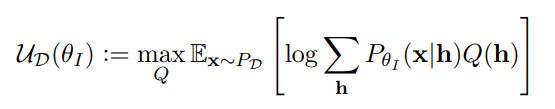
\includegraphics[width=\textwidth]{./arch_review_figs/mub.png}
\end{figure}

В работе~\cite{search_space} рассматриваются подходы к сэмплированию моделей глубокого обучения. Под \textit{сэмплированием} понимается порождение нескольких экземпляров модели из заданного распределения для дальнейшего выбора наилучшей модели. Предлагается формализация пространства поиска и формальное описание элементов  пространства моделей:
 \begin{figure}[H]
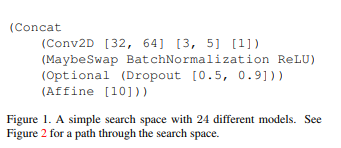
\includegraphics[width=\textwidth]{./arch_review_figs/search_space.png}
\end{figure}

\subsection{Метаоптимизация: learning to learn}
В работе~\cite{self_rnn} предлагается подход к адаптивному изменению структуры сети, основанный на обучении с подкреплением. Предлагается параметризация модели нейросети, включающая в себя модифицирующие и анализирующие выходы, позволяющие модифицировать параметры модели:
\begin{figure}[H]
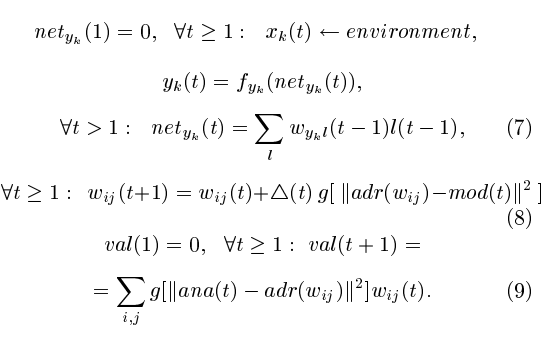
\includegraphics[width=\textwidth]{./arch_review_figs/self_rnn.png}
\end{figure}
Предлагается продолжение подхода, позволяющая рекуррентно продолжать анализ модели и порождать мета-мета-$\dots$-анализ.

В работе~\cite{meta_sgd} рассматривается оптимизация метапараметров (шага градиентного спуска и начального распределения параметров) с использованием обучения с подкреплением. На каждой итерации сэмплируется подвыборка, по которой проводится оптимизация данных метапараметров:
\begin{figure}[H]
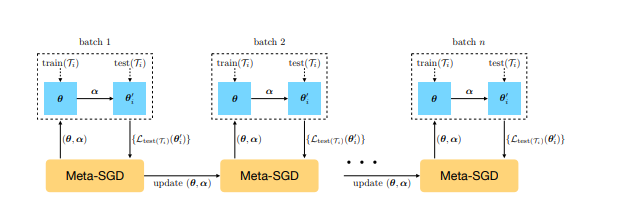
\includegraphics[width=\textwidth]{./arch_review_figs/meta_sgd.png}
\end{figure}

В работе~\cite{l2l} рассматирвается задача восстановления параметров модели по параметрам слабо обученной модели:
\begin{figure}[H]
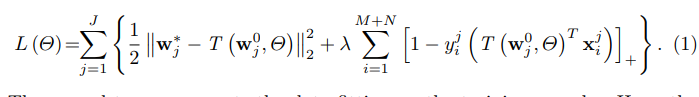
\includegraphics[width=\textwidth]{./arch_review_figs/l2l.png}
\end{figure}

\begin{figure}[H]
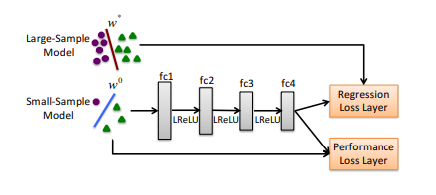
\includegraphics[width=\textwidth]{./arch_review_figs/l2l_scheme.png}
\end{figure}

В работе~\cite{l2l_by_gd_gd} рассматривается оптимизация метапараметров оптимизации с помощью LSTM, которая выступает альтернативе аналитических алгоритмов, таких как Adam или AdaGrad. LSTM имеет  (сравнительно) небольшое количество параметров, т.к. для каждого метапараметра используется своя копия модели LSTM с одинаковыми параметрами для каждой копии:
\begin{figure}[H]
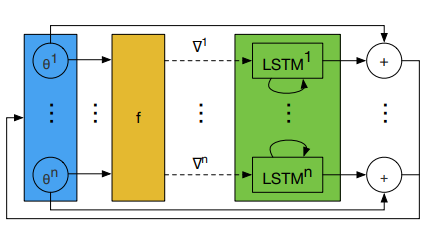
\includegraphics[width=\textwidth]{./arch_review_figs/l2lbygd.png}
\end{figure}




\subsection{Перебор структур}
В работе~\cite{search_smbo} рассматривается задача порождения сверточных нейронных сетей. Предлагается проводить поиск оптимальной структуры сети по восходящему по сложности порядку: начиная от сетей с одни блоком и наращивая блоки. В силу высокой вычислительной сложности данного подхода, вместо построения модели,предлагается обучить рекуррентную нейросеть,которая предсказывает качество модели по заданным блокам. 


В работе~\cite{optimal_racing} рассматривается задача выбора архитектуры с помощью большого количества параллельных запусков обучения моделей, предлагаются критерии ранней остановки оптимизации обучения моделей.


\subsection{ Обучение с подкреплением}
В работе~\cite{reinf} представлена схема выбора архитектуры сверточной нейросети с использованием обучения с подкреплением. В качестве актора (контроллера) выступает рекуррентная нейронная сеть.
\begin{figure}[H]
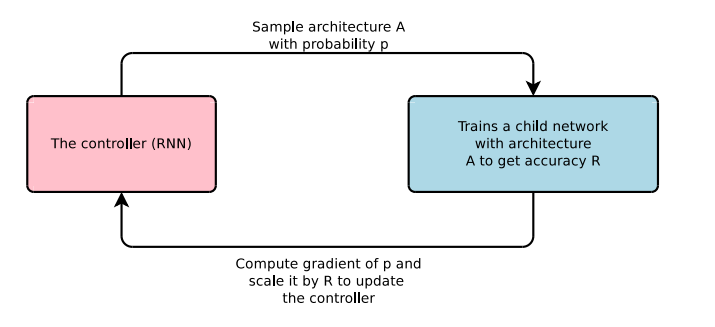
\includegraphics[width=\textwidth]{./arch_review_figs/reinf.png}
\end{figure}
В работе~\cite{reinf_predict} предлагается построение регрессионной модели для оценки финального качества модели и ранней остановки оптимизации моделей. Данный подход позволил существенно ускорить поиск моделей, представленный в работе~\cite{reinf}.
В работе~\cite{reinf_transfer} рассматривается задача переноса архитектуры нейросети, обученной на более простой выборки, на более сложную. Также предлагается параметризация пространства поиска, более делатьное, чем в~\cite{reinf}:
\begin{figure}[H]
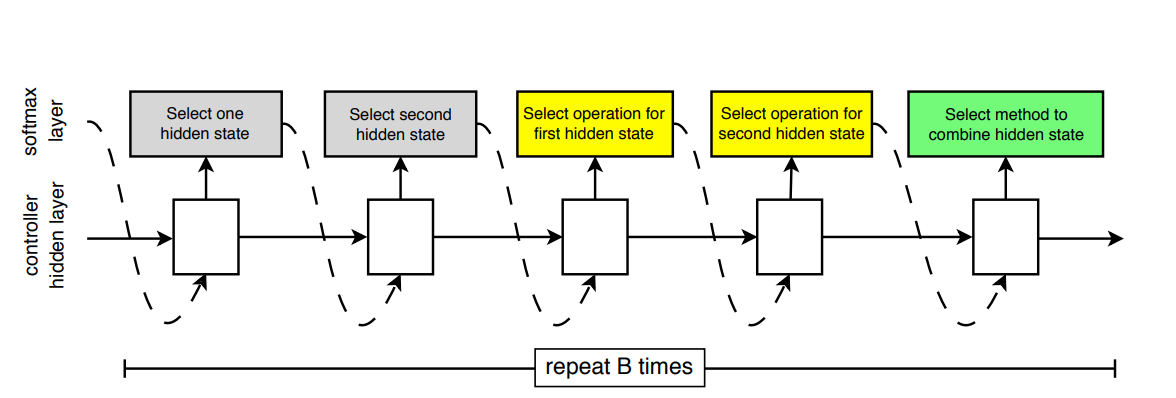
\includegraphics[width=\textwidth]{./arch_review_figs/reinf2.png}
\end{figure}

В отличие от предыдущих работ, в работе~\cite{reinf_deep2net} предлагается подход к инкрементальному обучению нейросети, основанном на модификации модели, полученной на предыдущем шаге. Рассматривается две операции над нейросетью:
\begin{itemize}
\item Расширение сети
\item Углубление сети
\end{itemize}

\begin{figure}[H]
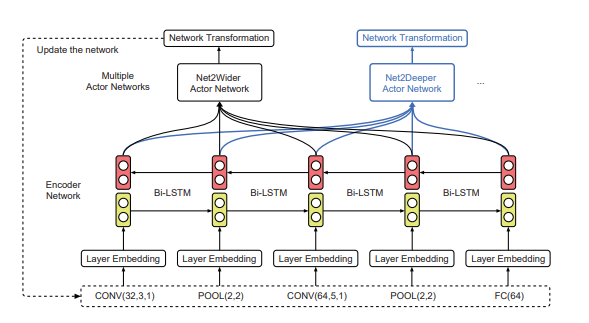
\includegraphics[width=\textwidth]{./arch_review_figs/deep2net.png}
\end{figure}



\section{Адаптивное изменение структуры}
В данном разделе собраны методы изменения структуры существующей модели. 

\textbf{Алгоритмы наращивания и прореживания параметров модели}
В работе~\cite{obd} предлагается удалять неинформативные параметры модели, где в качестве показателя информативности выступает следующий фнуционал: 
\begin{figure}[H]
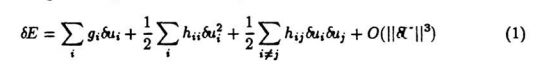
\includegraphics[width=\textwidth]{./arch_review_figs/obd.png}
\end{figure}
В работе~\cite{obs} было предложено развитие данного метода. В данной работе, в отличие от~\cite{obd} не вводится предположений о дигональности Гессиана функции ошибок, поэтому удаление неинформативных параметров модели производится точнее.

В работе~\cite{nips} был предложен метод, основанный на получении вариационной нижней оценки правдоподобия модели. В качестве критерия информативности параметра выступало отношение вероятности нахождения параметра в пределах априорного распределения к вероятности равенста параметра нулю:
\begin{figure}[H]
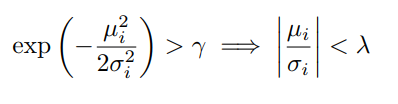
\includegraphics[width=\textwidth]{./arch_review_figs/nips_var.png}
\end{figure}
Идея данного метода была развита в~\cite{bayes_compr}, где также используются вариационные методы. В отличие от предыдущей работы, в данной работе рассматривается ряд априорных распределений параметров, позволяющих прореживать модели более эффективно:
\begin{itemize}
\item Нормальное распределение с лог-равномерным распределением дисперсии, независимой для каждого нейрона:
\begin{figure}[H]
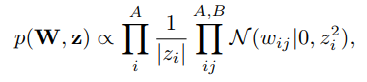
\includegraphics[width=\textwidth]{./arch_review_figs/bayes_compr_group.png}
\end{figure}
\item Произвденеие двух половинных распределений Коши: одно ответственно за отдельный параметр, другое --- за общее распределение параметров:
\begin{figure}[H]
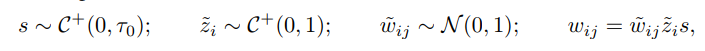
\includegraphics[width=\textwidth]{./arch_review_figs/bayes_compr_cauchy.png}
\end{figure}
\end{itemize}

Смежной темой к прореижванию моделей выступает компрессия нейросетей. Основным отличием задачи прореживания и компрессии выступает эксплуатационное требование: если прореживание используется для получения оптимальной и наиболее устойчивой модели, то компрессия часто производится для сохранения памяти и основных эксплуатационных характеристик исходной модели (?).
В работе~\cite{nvidia_prune}
предлагается итеритавиное использование регуляризации типа DropOut~\cite{dropout} для прореживания модели. 
В работах~\cite{weight_quantization, weight_quantization2} используются методы снижения вычислительной точности представления парамеров модели на основе кластеризации весов.
В работе~\cite{weight_quantization2} предлагается метод компрессии, основанный на кластеризации значений параметров модели и представлении их в сжатом виде на основе кодов Хаффмана.

В работах~\cite{boost_res, adanet} предлагается наращивание моделей, основанное на бустинге. В работе рассматривается задача построения нейросетевых моделей специального типа:
\[
    f_{t+1} = \sigma(f_t) + f_t,
\]
приводится параметризация модели, позволяющая рассматривать декомпозировать модель на слабые классификаторы.
В работе~\cite{adanet} на каждом шаге построения выбирается одно из двух расширений модели, каждое из которых рассматирвается как слабый классификатор:
1. Сделать модель шире
2. Сделать модель глубже
\begin{figure}[H]
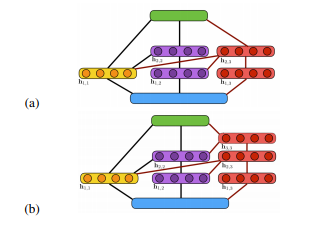
\includegraphics[width=0.5\textwidth]{./arch_review_figs/adanet.png}
\end{figure}
Построение модели заканчивается при условии снижении радемахереовской сложности:
\begin{figure}[H]
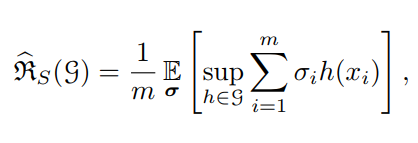
\includegraphics[width=0.5\textwidth]{./arch_review_figs/rad.png}
\end{figure}



\section{Байесовские методы порождения и выбора моделей}
\subsection{Автоматическое определение релевантности параметров}
В работе~\cite{hyper} рассматривается задача оптимизации гиперпараметров.  Авторы предлагают оптимизировать константы $l_2$-регуляризации отдельно для каждого параметра модели, проводится параллель с методами автоматического определения релевантности параметров (ARD)~\cite{MacKay}.

В работе~\cite{ard} рассматривается метод ARD для снижения размерности скрытого пространства вариационных порождающих моделей: скрытая переменная параметризуется как  произведение некоторой случайной величины $\mathbf{z}$  на вектор, отвечающий за релевантность каждой компоненты скрытой переменной:
\begin{figure}[H]
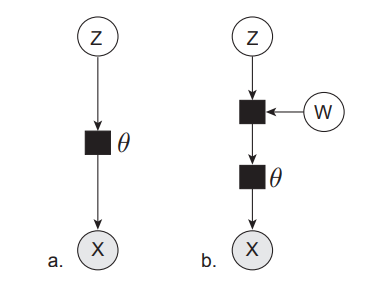
\includegraphics[width=0.5\textwidth]{./arch_review_figs/ard.png}
\end{figure}

\subsection{Суррогаты}
В работе~\cite{bo_gp} предлагается моделировать качество модели гауссовым процессом, параметрами которого выступают гиперпараметры исходной модели.
Модель, аппроксимирующая качество исходной модели, называется суррогатом. 

Одна из основных проблем использования гауссового процесса как суррогатной модели --- кубическая сложность оптимизации. В работе~\cite{random_gaus} предлагается использовать случайные подпространства гиперпараметров для ускоренной оптимизации.  В работе~\cite{gp_tree} предлагается кобминация из множества гауссовых моделей и линейной модели, позволяющая модели нелинейные зависимости гиперпараметров, а также существенно сократить сложность оптимизации. 

В работе~\cite{rbf_surrogate} предлагается рассматривать RBF-модель для аппроксимации качества исходной модели, что позволяет ускорить процесс оптимизации суррогатной модели. В~\cite{snoek_deep} рассматривается глубокая нейронная сеть в качестве суррогатной функции. Вместо интеграла правдоподобия, который оценивается в случае использования гауссового процесса в качестве суррогата, используется максимум апостериорной веротяности.

Важным параметром гауссовых процессов является функиия ядра гауссового процесса, полностью определяющая процесс в случае нулевого среднего. В работе~\cite{gp_fusion} предлагается функция ядра, определенная на графах:
    \[
    k(x,y) = r(d(x,y)),
    \]
где $d$ --- геодезическое расстояние между вершинами графа, $r$ --- некоторая вещественная функция (наверно положительно определенная, но это не указано явно в статье).
В работе~\cite{gp_arc} рассматривается задач выбора структуры нейросети, предлагается ядро специального вида, позволюящее учитывать только те гиперпапараметры, которые есть в обеих сравниваемых моделях: к примеру, для двуслойной и трехслойной нейросети будут уччитываться гиперпараметры, отвечающие только за первые два слоя. 
\begin{figure}[H]
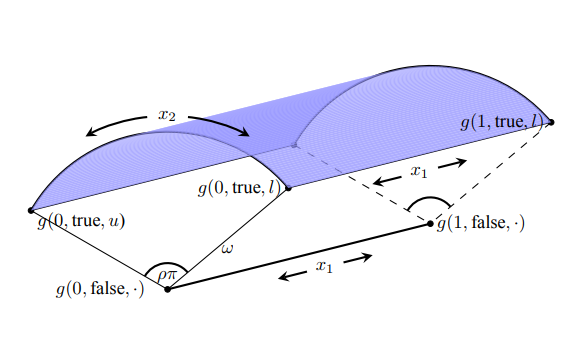
\includegraphics[width=0.5\textwidth]{./arch_review_figs/arc.png}
\end{figure}


\subsection{Адаптивное изменение структуры}

В работе~\cite{cib} рассматривается порождение unsupervised-моделей с использованием расширения процесса Индийского Буфета:
\begin{figure}[H]
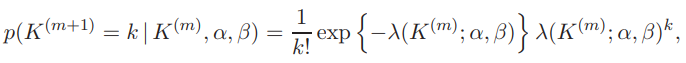
\includegraphics[width=0.5\textwidth]{./arch_review_figs/cib_eq.png}
\end{figure}
\begin{figure}[H]
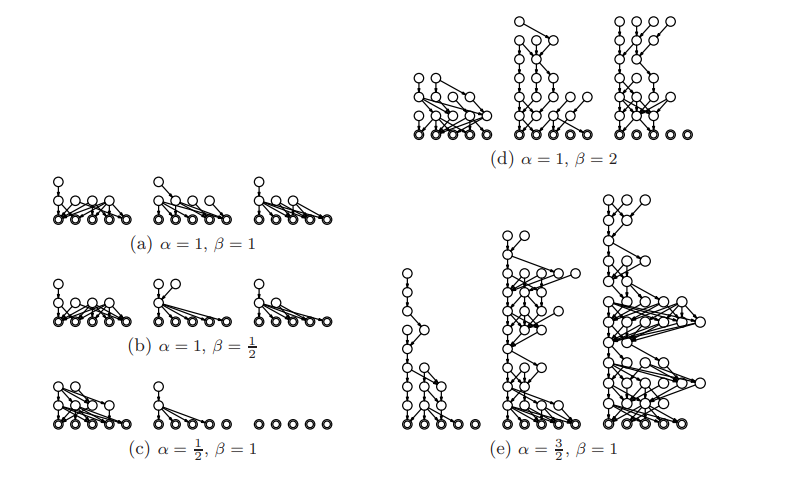
\includegraphics[width=0.5\textwidth]{./arch_review_figs/cib.png}
\end{figure}

В работе~\cite{cib_simple} предлагается упрощенная модель Индийского Буфета:
\begin{figure}[H]
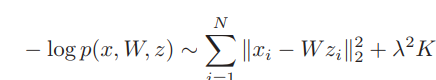
\includegraphics[width=0.5\textwidth]{./arch_review_figs/cib_simple.png}
\end{figure}

В работе~\cite{shirakawa2018dynamic} предлагается параметризация структуры модели с использованием Бернуллиевских величин:
каждая величина отвечает за включение или выключение слоя сети.



\subsection{Порождающие модели}
В работе~\cite{Kingma} было предложено обобщение вариационного автокодировщика на случай частичного обучения: 
итоговая модель вариационного автокодировщика является порождающей моделью, учитывающий метки объектов. 

В работе~\cite{vae_graph} рассматривается обобщение вариационного автокодировщика на случай более общих графических моделей. Рассматривается проводить оптимизацию сложных графических моделей в единой процедуре. Для вывода предлагается использовать нейронные сети.
Другая модификация вариационного автокодировщика представлена в работе~\cite{vae_stick}, авторы рассматривают использование процесса сломанной трости в вариационном автокодировщике, тем самым получая модель со стохастической размерностью скрытой переменной. В работе~\cite{vae_mix} рассматривается смесь автокодировщиков, где смесь моделируется процессом Дирихле.


В работе~\cite{var_boost} предлагается подход к оптимизации неизвестного распределения с помощью вариационного вывода. Авторы предлагают решать задачу оптимизации итеративно, добавляя в модель новые компоненты вариационного распределения, проводится аналогия с бустингом.
\subsection{Состязательные модели}

\section{Способы прогнозирования графовых структур}
В разделе собраны ключевые работы по порождению графовых моделей.

В работе~\cite{jaakkola2010learning} предлагается метод прогнозирования графовой структуры на основе линейного программирования. Предлагается свести проблему поиска графовой структуры к комбинаторной проблеме.

В работе~\cite{double_rnn} предлагается метод прогнозирования структур деревьев, основанный на дважды-рекуррентных нейросетях (doubly-reccurent), т.е. на сетях, отдельно предсказывающих глубину и ширину уровней деревьев.
\begin{figure}[H]
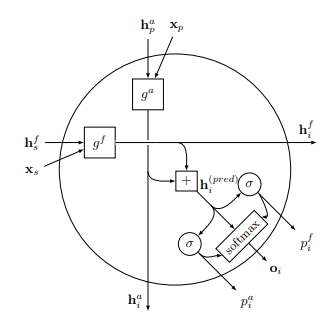
\includegraphics[width=0.5\textwidth]{./arch_review_figs/jaakkola.png}
\end{figure}


\section{Эвристические и прикладные методы}
\subsection{Эвристические методы}
В работе~\cite{layer_probe} предлагается метод анализа структуры сети на основе линейных классификаторов, построенных на промежуточных слоях нейросети.
Схожий метод был предложен в~\cite{branches}, где классификаторы на промежуточных уровнях используются для уменьшения вычислений при выполнении вывода и предсказаний.
Промежуточные классификаторы.работают как решающий список
http://www.eecs.harvard.edu/~htk/publication/2016-icpr-teerapittayanon-mcdanel-kung.pdf

В работе~\cite{nn_inc} предлагается инкрементальный метод построения нейросети: на каждом этапе построения в модель добавляются новые слои. Для улучшения качества модели, слои добавляются в начало модели, и затем проходят оптимизацию.

\subsection{Структуры сетей специального вида}
В данном разделе представлены работы по поиску оптимальной структуры сети, описывающие частные случаи поиска оптимальных моделей со структурами специального вида.

В работе~\cite{mixed} рассматривается оптимизация моделей нейросетей с бинарной функцией активацией. Задача оптимизации сводится к задаче mixed integer программирования, которая решается методами выпуклого анализа.


SKIP-сети, нужно ли писать? ResNet?
%https://papers.nips.cc/paper/6205-swapout-learning-an-ensemble-of-deep-architectures.pdf
%https://arxiv.org/pdf/1603.09382.pdf

%https://arxiv.org/pdf/1711.03130.pdf
В работе~\cite{energynet} предлагается метод построения сети глубокого обучения, структура которой выбирается с использованием обучения без учителя. Критерий оптимальности модели использует оценки энергитических функций и ограниченной машины Больцмана.

%https://arxiv.org/pdf/1511.02954.pdf
%https://arxiv.org/pdf/1701.08734.pdf
В работах~\cite{pathnet, supernet} рассматривается выбор архитектуры сети с использованием \textit{суперсетей}: больших связанных между собой сетей, образующих граф, пути в котором определяют итоговую архитектуру нейросети. В работе~\cite{supernet} рассматриваются стохастические суперсет, позволяющие выбрать структуру нейросети за органиченное время оптимизации. 
Схожий подход был предложен в работе~\cite{pathnet}, где предлагается использовать эволюционные алгоритмы для запоминания оптимальных подмоделей и переноса этих моделей в другие задачи.
\begin{figure}[H]
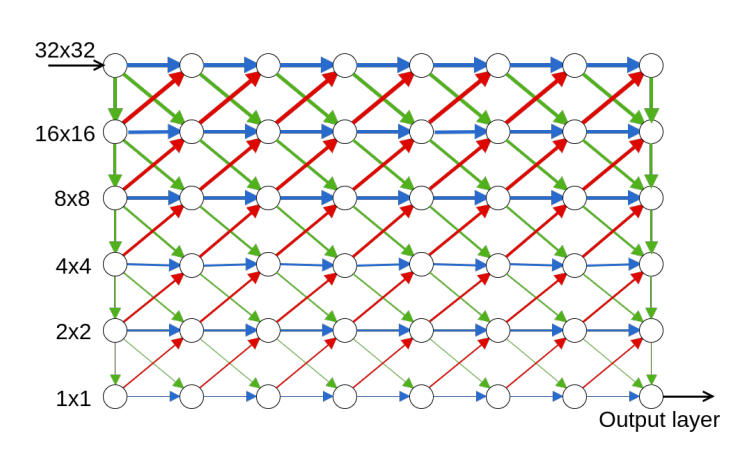
\includegraphics[width=0.5\textwidth]{./arch_review_figs/supernets.png}
\end{figure}

%https://arxiv.org/pdf/1511.02954.pdf 
%https://arxiv.org/pdf/1511.05641.pdf
%https://arxiv.org/pdf/1701.03281.pdf
В работах~\cite{net2net, morph, partition} рассматриваются методы деформации нейросетей. 
В работе~\cite{partition} предлагается метод оптимального разделения нейросети на несколько независимых сетей для уменьшения количества связей и, как следствие, уменьшения сложности оптимизации модели. В работе~\cite{net2net} предлагается метод сохранения результатов оптимизации нейросети при построении новой более глубокой или широкой нейросети. 
В работе~\cite{morph} рассматривается задача расширения сверточной нейросети, нейросеть рассматривается как граф.





\chapter{Выбор модели с использованием вариационного вывода}
\newpage{}
\addcontentsline{toc}{section}{Выбор модели с использованием вариационного вывода}
\chapter*{Выбор модели с использованием вариационного вывода}
Задана выборка  \begin{equation}\label{eq:dataset}\mathfrak{D} = \{(\mathbf{x}_i,y_i)\}, i = 1,\dots,m,\end{equation} состоящая из множества пар <<объект-метка>> $$\mathbf{x}_i \in \mathbf{X} \subset \mathbb{R}^n, \quad {y}_i \in \mathbf{y} \subset \mathbb{Y}.$$ Метка ${y}$  объекта $\mathbf{x}$ принадлежит либо множеству: ${y} \in \mathbb{Y} = \{1, \dots, Z\}$ в случае задачи классификации, где $Z$ --- число классов, либо некоторому подмножеству вещественных чисел ${y} \in \mathbb{Y}  \subseteq \mathbb{R}$ в случае задачи регрессии.

Моделью глубокого обучения $\mathbf{f}$ назовем суперпозицию функций
\begin{equation}
\label{eq:main}
 \mathbf{f}(\mathbf{w}, \mathbf{X}) = \mathbf{f}_1(\mathbf{f}_2(\dots \mathbf{f}_K(\mathbf{w}, \mathbf{X}))): \mathbb{R}^{m \times n} \to \mathbb{Y}^m,
\end{equation}
где $\mathbf{f}_k$ --- подмодели, параметрическое семейство дважды дифференцируемых по параметрам вектор-функций, $k \in \{1,\dots,K\}$; $\mathbf{w} \in \mathbb{R}^u$~---~вектор параметров моделей.\\
Для каждой модели определена функция правдоподобия  $p(\mathbf{y}|\mathbf{X}, \mathbf{w}, \mathbf{f})$, где $\mathbf{x}$ --- строка матрицы $\mathbf{X}$, $\mathbf{y}$ --- вектор меток зависимой переменной $y$.
Множество всех рассматриваемых моделей обозначим $\mathfrak{F}$. Для каждой модели $\mathbf{f}$ из конечного множества моделей $\mathfrak{F}$ задано априорное распределение параметров $p(\mathbf{w}|\mathbf{f})$.

%http://arxiv.org/pdf/math/0406221v1.pdf
Сложностью модели $\mathbf{f}$ назовем правдоподобие модели: %стохастическую сложность ее описания~\cite{mdl, grun2}:
%\[
%	\textnormal{C}(\mathbf{y},\mathbf{f}) = \textnormal{Len}(\mathbf{y}|\hat{\mathbf{w}}, \mathbf{f}) + \textnormal{COMP}(\mathbf{f}),
%\]
%где  $\textnormal{Len}(\mathbf{y}|\hat{\mathbf{w}}, \mathbf{f})$ --- \emph{длина описания} матрицы $\mathbf{y}$ с использованием модели $\mathbf{f}$ и оценки вектора %параметров $\hat{\mathbf{w}}$, полученных методом наибольшего правдоподобия, а $\textnormal{COMP}(\mathbf{f})$ --- величина, характеризующая \emph{параметрическую сложность} модели, т.е. способность модели описать произвольную выборки из $\mathbb{R}^n$~\cite{grun}.

%Байесовой интерпретацией сложности $\textnormal{C}$ является правдоподобие модели~\cite{MacKay}:
\begin{equation}
\label{eq:evidence}
	p(\mathbf{y}|\mathbf{X},\mathbf{f}) = \int_{\mathbf{w} \in \mathbb{R}^u} p(\mathbf{y}|\mathbf{X},\mathbf{w}, \mathbf{f})p(\mathbf{w}|\mathbf{f})d\mathbf{w}.
\end{equation}

Модели $\mathbf{f} \in \mathfrak{F}$ имеют различные размерности $u$ соответствующих векторов параметров. Также заданы различные априорные распределения их параметров $p(\mathbf{w}|\mathbf{f})$.
%Заметим, что в общем случае оценки правдоподобия модели и сложности модели могут различаться~\cite{grun}.


Модель классификации $\mathbf{f}$ назовем оптимальной среди моделей $\mathfrak{F}$, если достигается максимум интеграла~\eqref{eq:evidence}.



Требуется найти оптимальную модель $\mathbf{f}$ среди заданного множества моделей $\mathfrak{F}$, а также значения ее параметров $\mathbf{w}$, доставляющие максимум апостериорной вероятности
\begin{equation}
\label{eq:posterior}
	p(\mathbf{w}|\mathbf{y},\mathbf{X},\mathbf{f}) = \frac{p(\mathbf{y}|\mathbf{X}, \mathbf{w}, \mathbf{f})p(\mathbf{w}|\mathbf{f})}{p(\mathbf{y}|\mathbf{X}, \mathbf{f})}.
\end{equation}


%\begin{example_empty}
\textsl{П\,р\,и\,м\,е\,р~\,1.} Рассмотрим задачу линейной регрессии:
\[
	\mathbf{y} =\mathbf{X} \mathbf{w} + \boldsymbol{\varepsilon},\quad \boldsymbol{\varepsilon}  \sim \mathcal{N}(\mathbf{0},\mathbf{1}),\quad \mathbf{w} \sim  \mathcal{N}(\mathbf{0},\mathbf{A}^{-1}),
\]
где $\mathbf{A}$ --- диагональная матрица. 
Правдоподобие зависимой переменной имеет вид
\begin{equation}
\label{eq:example1}
	p(\mathbf{y}|  \mathbf{X}, \mathbf{w}, \mathbf{f}) = (2\pi) ^{-\frac{m}{2}} \textnormal{exp} \bigl(-\frac{1}{2}(\mathbf{y} -\mathbf{X} \mathbf{w})^\mathsf{T}(\mathbf{y} - \mathbf{X}\mathbf{w})\bigr),
\end{equation}
априорное распределение параметров модели имеет вид
\begin{equation}
\label{eq:prior}	
p(\mathbf{w}|\mathbf{f}) =  (2\pi) ^{-\frac{n}{2}} |\mathbf{A}|^{\frac{1}{2}} \textnormal{exp} (-\frac{1}{2}\mathbf{w}^\mathsf{T}\mathbf{A}\mathbf{w}).
\end{equation}

Правдоподобие модели~\eqref{eq:evidence} в этом примере вычисляется аналитически~\cite{hyperopt}:
\begin{equation}
\label{eq:ground}
	p(\mathbf{y}|\mathbf{X},\mathbf{f})  =  (2\pi) ^{-\frac{m}{2}} |\mathbf{A}|^{\frac{1}{2}} |\mathbf{H}|^{-\frac{1}{2}}  \textnormal{exp}\bigl(-\frac{1}{2}(\mathbf{y} -\mathbf{X} \hat{\mathbf{w}})^\mathsf{T}(\mathbf{y} - \mathbf{X}\hat{\mathbf{w}})\bigr)\textnormal{exp} \bigl(-\frac{1}{2}\hat{\mathbf{w}}^\mathsf{T}\mathbf{A}\hat{\mathbf{w}}\bigr),
\end{equation}
где $\hat{\mathbf{w}}$ --- значение наиболее вероятных~\eqref{eq:posterior} параметров модели:
\[
	\hat{\mathbf{w}} = \argmax p(\mathbf{w}|\mathbf{y}, \mathbf{X}, \mathbf{f}) = (\mathbf{A} + \mathbf{X}^\mathsf{T}\mathbf{X})^{-1}\mathbf{X}^\mathsf{T}\mathbf{y},
\]
$\mathbf{H}$ --- гессиан функции потерь $L$ модели:
\[
	\mathbf{H}	= \nabla \nabla_\mathbf{w} \left(\frac{1}{2} (\mathbf{y} -\mathbf{X} {\mathbf{w}})^\mathsf{T}(\mathbf{y} - \mathbf{X}{\mathbf{w}}) + \frac{1}{2}\mathbf{w}^\mathsf{T}\mathbf{A}\mathbf{w} \right) = \mathbf{A} + \mathbf{X}^\mathsf{T}\mathbf{X},
\]

\[ 
	L = - \textnormal{log} p(\mathbf{y}|  \mathbf{X}, \mathbf{w}, \mathbf{f}). 
\]
%\end{example_empty}

%\paragraph{Пример 2.} Рассмотрим задачу классификации, в которой модель --- нейросеть с softmax-слоем на выходе:
%\[
%\mathbf{f} = \mathbf{f}_\textnormal{SM}(\mathbf{f}_2(\dots \mathbf{f}_K(\mathbf{x}))),
%\]
%$\mathbf{f}_2, \dots, \mathbf{f}_K$ --- дифференцируемые функции, $\mathbf{f}_\textnormal{SM}$ --- многомерная логистическая функция:
%\[
%	\mathbf{f}_\textnormal{SM} = \frac{\mathbf{f}_2(\dots \mathbf{f}_K(\mathbf{x}))}{\sum_{r=1}^Z \textnormal{exp}\bigl( {f}_{r,2}(\dots \mathbf{f}_K(\mathbf{x})) \bigr)},
%\]
%где ${f}_{r,2}$ --- $r$-я компонента функции $\mathbf{f}_2$. Компонента $r$ вектора $\mathbf{f}_\textnormal{SM}$ определяет вероятность принадлежности объекта $\mathbf{x}$ к классу $r$. Логарифм правдоподобия зависимой переменной аналогично~\eqref{eq:example1} имеет вид
%\[
%	\textnormal{log} p({y}|\mathbf{x}, \mathbf{w}, \mathbf{f}) =  \textnormal{log}~\hat{f}_{\hat{r},\textnormal{SM}} (\mathbf{f}_2(\dots \mathbf{f}_K(\mathbf{x}))),
%\]
%где $\hat{f}_{\hat{r},\textnormal{SM}}$ соответствует ненулевой компоненте вектора ${y}$:
%$$\hat{r} \in \{1,\dots,Z\}: y_{r} >0,$$
%$y_{r}$ --- компонента вектора ${y}$. 

%-Интеграл правдоподобия~\eqref{eq:evidence} модели является трудновычислимым для данного семейства моделей. Одним из методов вычисления приближенного значения правдоподобия является получение вариационной оценки правдоподобия.  


{В качестве функции, приближающей логарифм интеграла~\eqref{eq:evidence}, будем рассматривать его нижнюю оценку, полученную при помощи неравенства Йенсена~\cite{Bishop}. Получим нижнюю оценку логарифма правдоподобия модели, используя неравенство}
\begin{equation} 
\label{eq:elbo}
\textnormal{log}~p(\mathbf{y}|\mathbf{X},\mathbf{f})  = \int_{\mathbf{w}} q(\mathbf{w})\textnormal{log}~\frac{p(\mathbf{y},\mathbf{w}|\mathbf{X},\mathbf{f})}{q(\mathbf{w})}d\mathbf{w} + \textnormal{D}_\textnormal{KL}  \bigl(q(\mathbf{w})||p(\mathbf{w}|\mathbf{y}, \mathbf{X}, \mathbf{f})\bigr) \geq	
\end{equation} 
$$
\geq \int_{\mathbf{w}} q(\mathbf{w})\textnormal{log}~\frac{p(\mathbf{y},\mathbf{w}|\mathbf{X},\mathbf{f})}{q(\mathbf{w})}d\mathbf{w} =
$$

$$
= -\textnormal{D}_\textnormal{KL} \bigl(q(\mathbf{w})||p(\mathbf{w}|\mathbf{f})\bigr) + \int_{\mathbf{w}} q(\mathbf{w})\textnormal{log}~{p(\mathbf{y}|\mathbf{X},\mathbf{w},\mathbf{f})} d \mathbf{w},
$$
где $\textnormal{D}_\textnormal{KL}\bigl(q(\mathbf{w})||p(\mathbf{w} |\mathbf{f})\bigr)$ --- расстояние Кульбака--Лейблера между двумя распределениями: $$\textnormal{D}_\textnormal{KL}\bigl(q(\mathbf{w})||p(\mathbf{w} |\mathbf{f})\bigr) = -\int_{\mathbf{w}} q(\mathbf{w})\textnormal{log}~\frac{p(\mathbf{w} | \mathbf{f})}{q(\mathbf{w})}d\mathbf{w},$$
$$
p(\mathbf{y},\mathbf{w}|\mathbf{X},\mathbf{f}) = p(\mathbf{y}|\mathbf{X},\mathbf{f})p(\mathbf{w}|\mathbf{f}).
$$

{
Вариационной оценкой логарифма правдоподобия модели~\eqref{eq:evidence} $\textnormal{log}~p(\mathbf{y}|\mathbf{X},\mathbf{f})$ называется оценка $\textnormal{log}~\hat{p}(\mathbf{y}|\mathbf{X},\mathbf{f})$, полученная аппроксимацией неизвестного апостериорного распределения $p(\mathbf{w}| \mathbf{y}, \mathbf{X}, \mathbf{f})$ заданным распределением $q(\mathbf{w})$.

}


Будем рассматривать задачу нахождения вариационной оценки как задачу оптимизации. Пусть задано множество распределений $Q =\{q(\mathbf{w})\}$. Сведем задачу нахождения наиболее близкой вариационной нижней оценки интеграла~\eqref{eq:evidence} к оптимизации вида
\[
     \hat{q}(\mathbf{w}) = \argmax_{q \in Q}  \int_{\mathbf{w}} q(\mathbf{w})\textnormal{log}~\frac{p(\mathbf{y},\mathbf{w}|\mathbf{X},\mathbf{f})}{q(\mathbf{w})}d\mathbf{w}.
\]  
В данной работе в качестве множества $Q$ рассматривается нормальное распределение и распределение параметров, неявно получаемое оптимизацией градиентными методами. 

Оценка~\eqref{eq:elbo} является нижней, поэтому может давать некорректные оценки для правдоподобия~\eqref{eq:evidence}. Для того, чтобы оценить величину этой ошибки, докажем следующее утверждение.

\label{st:st1} Пусть задано множество $Q = \{q(\mathbf{w})\}$ непрерывных распределений. Максимизация вариационной нижней оценки $$\int_{\mathbf{w}} q(\mathbf{w})\textnormal{log}~\frac{p(\mathbf{y},\mathbf{w}|\mathbf{X},\mathbf{f})}{q(\mathbf{w})}d\mathbf{w}$$  логарифма интеграла~\eqref{eq:evidence}  эквивалентна минимизации расстояния Кульбака--Лейблера между распределением $q(\mathbf{w}) \in Q$ и апостериорным распределением параметров $p(\mathbf{w}|\mathbf{y}, \mathbf{X}, \mathbf{f})$:
\begin{equation}
\label{eq:optim}
    \hat{q} = \argmax_{q \in Q} \int_{\mathbf{w}} q(\mathbf{w})\textnormal{log}~\frac{p(\mathbf{y},\mathbf{w}|\mathbf{X},\mathbf{f})}{q(\mathbf{w})}d\mathbf{w} \Leftrightarrow 	
    \hat{q} = \argmin_{q \in Q} \textnormal{D}_\textnormal{KL}  \bigl(q(\mathbf{w})||p(\mathbf{w}|\mathbf{y}, \mathbf{X}, \mathbf{f})\bigr),
\end{equation}

\[
	\textnormal{D}_\textnormal{KL}  \bigl(q(\mathbf{w})||p(\mathbf{w}|\mathbf{y}, \mathbf{X}, \mathbf{f})\bigr) =  \int_\mathbf{w} q(\mathbf{w}) \frac{q(\mathbf{w})}{p(\mathbf{w}|\mathbf{y}, \mathbf{X}, \mathbf{f})} d\mathbf{w}.
\]


Таким образом, задача нахождения вариационной оценки, близкой к значению интеграла~\eqref{eq:evidence} сводится к поиску распределения $\hat{q}$, аппроксимирующего распределение $p(\mathbf{w}|\mathbf{y}, \mathbf{X}, \mathbf{f})$ наилучшим образом. Доказательство утверждения~1 см. в Приложении.

Модель $\mathbf{f}$ назовем субоптимальной на множестве моделей $\mathfrak{F}$  по множеству распределений ${Q}$, если модель доставляет максимум нижней вариационной оценке интеграла~\eqref{eq:optim}
\begin{equation}
\label{eq:elbo2}
	\max_{q \in {Q}}\int_{\mathbf{w}} q(\mathbf{w})\textnormal{log}~\frac{p(\mathbf{y},\mathbf{w}|\mathbf{X},\mathbf{f})}{q(\mathbf{w})}d\mathbf{w}.
\end{equation}


{
Субоптимальность модели может быть также названа вариационной оптимальностью модели или LB-оптимальностью (\textit{Lower Bound --- нижняя граница}) модели.}

Вариационная оценка~\eqref{eq:elbo} интерпретируется как оценка сложности модели по принципу минимальной длины описания~\cite{mdl}, где первое слагаемое определяет количество информации для описания выборки, а второе слагаемое --- длину описания самой модели~\cite{nips}.
%\[
%	\textnormal{MDL}(\mathbf{y},\mathbf{f}) = \textnormal{Len}(\mathbf{y}|\hat{\mathbf{w}}, \mathbf{f}) + \textnormal{COMP}(\mathbf{f}),
%\]
%где  $\textnormal{Len}(\mathbf{y}|\hat{\mathbf{w}}, \mathbf{f})$ --- \emph{длина описания} матрицы $\mathbf{y}$ с использованием модели $\mathbf{f}$ и оценки вектора %параметров $\hat{\mathbf{w}}$, полученных методом наибольшего правдоподобия, а $\textnormal{COMP}(\mathbf{f})$ --- величина, характеризующая \emph{параметрическую сложность} модели, т.е. способность модели описать произвольную выборки из $\mathbb{R}^n$~\cite{grun}.


В данной работе решается задача выбора субоптимальной модели при различных заданных множествах $Q$.

\section{Методы получения вариационной оценки правдоподобия}
Ниже представлены методы получения вариационных нижних оценок~\eqref{eq:elbo2} правдоподобия~\eqref{eq:evidence}. В первом подразделе рассматривается метод, основанный на аппроксимации апостериорного распределения $p( \mathbf{w}|\mathbf{y}, \mathbf{X}, \mathbf{f})$~\eqref{eq:posterior} многомерным гауссовым распределением с диагональной матрицей ковариаций. В последующих разделах рассматриваются методы, основанные на различных модификациях стохастического градиентного спуска. 

\subsection{Аппроксимация нормальным распределением}
В качестве множества $Q = \{q(\mathbf{w})\}$ задано параметрическое семейство нормальных распределений с диагональными матрицами ковариаций:
\begin{equation}
\label{eq:diag}
	q \sim \mathcal{N}(\boldsymbol{\mu}_q, \mathbf{A}^{-1}_q),
\end{equation}
где $\mathbf{A}_q$ --- диагональная матрица ковариаций, $\boldsymbol{\mu}_q$ --- вектор средних компонент.

Пусть априорное распределение $p(\mathbf{w}|\mathbf{f})$~\eqref{eq:prior} параметров модели задано как нормальное:
\[
	p(\mathbf{w}|\mathbf{f}) \sim \mathcal{N}(\boldsymbol{\mu}, \mathbf{A}^{-1}).
\] 
Тогда оптимизация~\eqref{eq:optim} имеет вид
\begin{equation}
\label{eq:norm_max}
 \int_{\mathbf{w}} q(\mathbf{w})\textnormal{log}~{p(\mathbf{y}|\mathbf{X},\mathbf{w},\mathbf{f})} d \mathbf{w} - D_\textnormal{KL}\bigl(q (\mathbf{w} )|| p (\mathbf{w}|\mathbf{f})\bigr) \to \max_{\mathbf{A}_q, \boldsymbol{\mu}_q},
\end{equation}
где расстояние $D_\textnormal{KL}$ между двумя гауссовыми величинами рассчитывается как 
\[
	D_\textnormal{KL}\bigl(q (\mathbf{w}) || p (\mathbf{w}|\mathbf{f})\bigr) = \frac{1}{2} \bigl( \textnormal{Tr} [\mathbf{A}\mathbf{A}^{-1}_q] + (\boldsymbol{\mu} - \boldsymbol{\mu}_q)^\mathsf{T}\mathbf{A}(\boldsymbol{\mu} - \boldsymbol{\mu}_q) - u +\textnormal{ln}~|\mathbf{A}^{-1}| - \textnormal{ln}~|\mathbf{A}_q^{-1}| \bigr).
\]
В качестве приближенного значения интеграла $$\int_{\mathbf{w}} q(\mathbf{w})\textnormal{log}~{p(\mathbf{y}|\mathbf{X},\mathbf{w},\mathbf{f})} d \mathbf{w}$$ предлагается использовать формулу
\[
\int_{\mathbf{w}} q(\mathbf{w})\textnormal{log}~{p(\mathbf{y}|\mathbf{X},\mathbf{w},\mathbf{f})} d \mathbf{w} \approx \sum_{i=1}^m \textnormal{log}~p({y}_i|\mathbf{x}_i, \mathbf{w}_i),
\]
где $\mathbf{w}_i$  --- реализация случайной величины из распределения $q(\mathbf{w})$.

Итоговая функция оптимизации~\eqref{eq:norm_max} имеет вид
\begin{equation}
\label{eq:gaus}
	\mathbf{f} = \argmax_{\mathbf{A}_q, \boldsymbol{\mu}_q} \sum_{i=1}^m \textnormal{log}~p({y}_i|\mathbf{x}_i, \mathbf{w}_i) - D_\textnormal{KL}\bigl(q (\mathbf{w} )|| p (\mathbf{w}|\mathbf{f})\bigr).
\end{equation}

%\begin{example_empty} 
%\hspace{\parindent}
\textsl{П\,р\,и\,м\,е\,р~\,2.}
Пусть  задана выборка $\mathfrak{D}$, в которой переменная ${y}$ не зависит от $\mathbf{x}$:
\begin{equation}
\label{eq:example_post}
	{y} \sim \mathcal{N}(\mathbf{w}, \mathbf{B}^{-1}),
\end{equation}

\[
	\mathbf{B}^{-1} = \left( \begin{array}{cc}
	2 & 1,8 \\
	1,8 & 2\\
	\end{array}  \right),
\]
\[
	p(\mathbf{w}|\mathbf{f}) = \mathcal{N}(\mathbf{0}, \mathbf{I}).
\]

График аппроксимации распределения параметров представлен на рис.~\ref{fig:var},\textit{а}. Как видно из графика, с использованием метода~\eqref{eq:gaus} получено грубое приближение апостериорного распределения $p(\mathbf{w}|\mathbf{y}, \mathbf{X}, \mathbf{f})$, что может существенно занизить оценку правдоподобия модели.



{Данный пример показывает, что качество итоговой аппроксимации распределения $p(\mathbf{w}|\mathbf{y}, \mathbf{X}, \mathbf{f})$ значительно зависит от схожести распределений $\hat{q}$ и $p(\mathbf{w}|\mathbf{y}, \mathbf{X}, \mathbf{f})$. В силу диагональности матрицы $\mathbf{A}_q$ и полного ранга матрицы $\mathbf{B}$  итоговое распределение $\hat{q}$ не может адекватно приблизить данное распределение  $p(\mathbf{w}|\mathbf{y}, \mathbf{X}, \mathbf{f})$.}



%\end{example_empty}
\subsection{Аппроксимация с использованием градиентного метода}
В качестве множества распределений $Q = \{q(\mathbf{w})\}$, аппроксимирующих неизвестное распределение $\textnormal{log}~p(\mathbf{y}|\mathbf{X},\mathbf{f})$, используются распределения параметров, полученные в ходе их оптимизации. 

Представим неравенство~\eqref{eq:elbo}
\begin{equation}
\label{eq:elbo_entropy}
 \textnormal{log}~p(\mathbf{y}|\mathbf{X},\mathbf{f}) \geq \int_\mathbf{w} q(\mathbf{w})\textnormal{log}~\frac{p(\mathbf{y},\mathbf{w}|\mathbf{X}, \mathbf{f})}{q(\mathbf{w})}d\mathbf{w} =  \mathsf{E}_{q(\mathbf{w)}}\bigl(\textnormal{log~}p (\mathbf{y}, \mathbf{w}|\mathbf{X}, \mathbf{f})\bigr) - \mathsf{S}\bigl({q(\mathbf{w)}}\bigr),
\end{equation}
где $\mathsf{S}$ --- энтропия распределения:
\[
\mathsf{S}\bigl({q(\mathbf{w)}}\bigr) = - \int_{\mathbf{w}} q(\mathbf{w})\textnormal{log}~q(\mathbf{w})d\mathbf{w},
\]
$$p (\mathbf{y}, \mathbf{w}|\mathbf{X}, \mathbf{f}) = p (\mathbf{w}| \mathbf{f}) p (\mathbf{y}|\mathbf{X}, \mathbf{w}, \mathbf{f}),$$
$\mathsf{E}_{q(\mathbf{w)}}\bigl(\textnormal{log~}p (\mathbf{y}, \mathbf{w}|\mathbf{X}, \mathbf{f})\bigr)$ --- матожидание логарифма вероятности $\textnormal{log~}p (\mathbf{y}, \mathbf{w}|\mathbf{X}, \mathbf{f})$:
\[
	\mathsf{E}_{q(\mathbf{w)}}\bigl(\textnormal{log~}p (\mathbf{y}, \mathbf{w}|\mathbf{X}, \mathbf{f})\bigr) = \int_\mathbf{w} \textnormal{log~}p (\mathbf{y}, \mathbf{w}|\mathbf{X}, \mathbf{f}) q(\mathbf{w}) d\mathbf{w}.
\]

Оценка распределений производится при оптимизации параметров. Оптимизация выполняется в режиме мультистарта~\cite{multi}, т.е. при запуске оптимизации параметров модели из нескольких разных начальных приближений. Основная проблема такого подхода~---~вычисление энтропии $\mathsf{S}$ распределений $q(\mathbf{w}) \in Q$. Ниже представлен метод получения оценок энтропии~\eqref{eq:entropy} ~$\mathsf{S}$ и оценок правдоподобия~\eqref{eq:elbo_entropy}.

Запустим $r$ процедур оптимизаций модели $\mathbf{f}$ из разных начальных приближений:
\[
	L(\mathbf{w}^1, \mathbf{y}, \mathbf{X}), \dots, L(\mathbf{w}^r, \mathbf{y}, \mathbf{X}) \to \min,
\] 
где $r$ --- число оптимизаций, $L$ --- оптимизируемая функция потерь
\begin{equation}
\label{eq:loss_func}
L = -\sum_{i=1}^m \textnormal{log}p({y}_i, \mathbf{w} |\mathbf{x}_i, \mathbf{f}) = -\textnormal{log}~p(\mathbf{w}|\mathbf{f}) - \sum_{i=1}^m \textnormal{log}p({y}_i |\mathbf{x}_i, \mathbf{w}, \mathbf{f}).
\end{equation}

Пусть начальные приближения параметров $\mathbf{w}^1, \dots, \mathbf{w}^r$ порождены из некоторого начального распределения $q^0(\mathbf{w})$:
\[
	\mathbf{w}^1, \dots, \mathbf{w}^r \sim q^0(\mathbf{w}). 
\]

%Обозначим за  $\mathbf{w}^g, g \in \{1,\dots,r\}$ значения параметров $\mathbf{w}^1, \dots, \mathbf{w}^r$ на  текущем шаге оптимизации. 

Для описания произвольного градиентного метода оптимизации параметров модели введем понятие оператора оптимизации. Оно используется для вычисления оценки энтропии распределения, полученного под действием этой оптимизации.

Назовем оператором оптимизации алгоритм $T$ выбора вектора параметров $\mathbf{w}'$  по параметрам предыдущего шага $\mathbf{w}$:
\[
	\mathbf{w}' = T(\mathbf{w}).
\]


Рассмотрим оператор градиентного спуска:
\begin{equation}
\label{eq:sgd}
	T(\mathbf{w}) = \mathbf{w} - \gamma \nabla L(\mathbf{w}, \mathbf{y}, \mathbf{X}), 
\end{equation}
где  $\gamma$ --- длина шага градиентного спуска.

Пусть значения $\mathbf{w}^1, \dots, \mathbf{w}^r$  --- реализации случайной величины из некоторого распределения $q(\mathbf{w})$. Начальная энтропия распределения $q(\mathbf{w})$ соответствует энтропии распределения $q^0(\mathbf{w})$, из которого были порождены начальные приближения оптимизации параметров $\mathbf{w}^1, \dots, \mathbf{w}^r$. Под действием оператора $T$ распределение параметров $\mathbf{w}_1, \dots, \mathbf{w}_r$ изменяется. Для учета энтропии распределений, полученных в ходе оптимизации,
{ формализуем метод,  представленный в~\cite{early}. }

~Пусть $T$ --- оператор градиентного спуска,
 $L$ --- функция потерь, градиент $\nabla L$ которой имеет константу Липшица $C_L$.  Пусть $\mathbf{w}^1,\dots,\mathbf{w}^r$ ---  начальные приближения оптимизации модели, где $r$ --- число начальных приближений. Пусть $\gamma$ --- длина шага градиентного спуска, такая что
\begin{equation}
\label{eq:ineq}
\gamma<\frac{1}{C_L}, \quad \gamma < \bigl(\max_{g \in \{1,\dots,r\}}\lambda_\textnormal{max} (\mathbf{H}(\mathbf{w}^g))\bigr)^{-1}, 
\end{equation}
где $\lambda_\textnormal{max}$ --- наибольшее по модулю собственное значение гессиана  $\mathbf{H}$ функции потерь $L$.

При выполнении неравенств~\eqref{eq:ineq} разность энтропий распределений $q'(\mathbf{w}), q(\mathbf{w})$ на смежных шагах почти наверное сходится к следующему выражению: 
\begin{equation}
\label{eq:entropy}
	\mathsf{S}\bigl(q'(\mathbf{w})) -  \mathsf{S}\bigl(q(\mathbf{w}))  \approx  \frac{1}{r}\sum_{g=1}^r \bigl(-\gamma \textnormal{Tr}[\mathbf{H}(\mathbf{w}'^g)] - \gamma \textnormal{Tr}[\mathbf{H}(\mathbf{w}'^g)\mathbf{H}(\mathbf{w}'^g)]  \bigr) + o_{\gamma^2 \to 0}(1),
\end{equation}
где $\mathbf{H}$ --- гессиан функции потерь $L$.


Получим итоговую формулу для оценки правдоподобия модели.

Оценка~\eqref{eq:elbo_entropy} на шаге оптимизации $\tau$ представима в виде
\begin{equation}
\label{eq:ev_grad_full}
\textnormal{log}~\hat{p}(\mathbf{y}|\mathbf{X}, \mathbf{f}) \approx \frac{1}{r} \sum_{g = 1}^r L(\mathbf{w}^g_\tau, \mathbf{X}, \mathbf{y})  + \mathsf{S}\big(q^0(\mathbf{w})\bigr) + \frac{1}{r}\sum_{b=1}^\tau\sum_{g=1}^r \bigl(-\gamma \textnormal{Tr}[\mathbf{H}(\mathbf{w}_b^g)] - \gamma^2 \textnormal{Tr}[\mathbf{H}(\mathbf{w}_b^g)\mathbf{H}(\mathbf{w}_b^g)]  \bigr) 
\end{equation}
с точностью до слагаемых вида $o_{\gamma^2 \to 0}(1)$,
где $\mathbf{w}_b^g$ --- $g$-я реализация параметров модели на шаге оптимизации $b$, $q^0(\mathbf{w})$ --- начальное распределение.



В~\cite{early} предлагается алгоритм приближенного вычисления для выражения, находящегося под знаком суммы в~\eqref{eq:ev_grad_full}:
\[
	-\gamma \textnormal{Tr}[\mathbf{H}(\mathbf{w}^g)] - \gamma^2 \textnormal{Tr}[\mathbf{H}(\mathbf{w}^g)\mathbf{H}(\mathbf{w}^g)]  \approx \mathbf{r}_0^\mathsf{T}\bigl(-2\mathbf{r}_0 + 3\mathbf{r}_1 -\mathbf{r}_2\bigr),
\]
где вектор $\mathbf{r}_0$  порождается из нормального распределения:
$$\mathbf{r}_0 \sim \mathcal{N}(\mathbf{0}, \mathbf{I}), \quad \mathbf{r}_1 = \mathbf{r}_0 - \gamma \mathbf{r}_0^\mathsf{T} \nabla \nabla L, \quad \mathbf{r}_2 = \mathbf{r}_1 - \gamma \mathbf{r}_1^\mathsf{T} \nabla \nabla L.$$


Заметим, что при приближении параметров модели к точке экстремума оценка правдоподобия устремляется в минус бесконечность в силу постоянно убывающей энтропии. Таким образом, чем ближе градиентный метод приближает параметры модели к точке экстремума, тем менее точной становится оценка правдоподобия модели. Один из методов борьбы с данной проблемой будет представлен в разделе 3.3.
Доказательство теоремы и утверждения 2 см. в Приложении.
%\begin{figure}
%\caption{Псевдокод алгоритма получения вариационной нижней оценки правдоподобия модели с использованием градиентного спуска}
%\label{fig:algo}
%\begin{algorithmic}[1]
%\REQUIRE $\mathbf{X}, \mathbf{y}, p(\mathbf{w}|\mathbf{f})$;
%\REQUIRE критерий останова $M$, начальное распределение параметров $q_0$, количество точек мультистарта $r$, функция потерь $L$, ее первая и вторая производные;
%\ENSURE $\textnormal{log}~\hat{p}(\mathbf{y}|\mathbf{X}, \mathbf{f})$;
%\FOR{$g=1,\dots,r$}
%\STATE $\mathbf{w}^g \sim q_0$;
%\ENDFOR
%\STATE $\mathsf{S} = \mathsf{S}\bigl(q_0)$;
%\WHILE{не достигнут критерий останова $M$}

%\FOR{$g=1,\dots,r$}
%\STATE $\mathbf{w}^g =  \mathbf{w}^g - \nabla L$;
%\STATE $\mathbf{r}_0 \sim \mathcal{N}(\mathbf{0}, \mathbf{I})$;
%\STATE $\mathbf{r}_1 = \mathbf{r}_0 - \gamma \mathbf{r}^{\mathsf{T}}_0 \nabla \nabla L(\mathbf{w}^g, \mathbf{y}, \mathbf{X})$;
%\STATE $\mathbf{r}_2 = \mathbf{r}_1 - \gamma \mathbf{r}^{\mathsf{T}}_1 \nabla \nabla L(\mathbf{w}^g, \mathbf{y}, \mathbf{X})$;
%\STATE $\mathsf{S}^g = \mathbf{r}_0^\mathsf{T}\bigl(-2\mathbf{r}_0 + 3\mathbf{r}_1 -\mathbf{r}_2\bigr)$;
%\ENDFOR
%\STATE $\mathsf{S} = \frac{1}{r}\sum_{g=1}^r \mathsf{S}^g$;
%\ENDWHILE
%\STATE $\hat{p}(\mathbf{y}|\mathbf{X}, \mathbf{w}, \mathbf{f}) = \frac{1}{r}\sum_{g=1}^r p(\mathbf{y}|\mathbf{X}, \mathbf{w}^g, \mathbf{f})$;
%\STATE $\hat{p}(\mathbf{w} | \mathbf{f}) = \frac{1}{r}\sum_{g=1}^r p(\mathbf{w}^g| \mathbf{f})$;
%\STATE $\textnormal{log}~\hat{p}(\mathbf{y}|\mathbf{X}, \mathbf{f}) = \textnormal{log}~\hat{p}(\mathbf{y}|\mathbf{X}, \mathbf{w}, \mathbf{f}) +\textnormal{log}~\hat{p}(\mathbf{w} | \mathbf{f})$;
	
%\end{algorithmic}
%\end{figure}


 
%\paragraph{Теорема 2.} Пусть выполнены условия Теоремы 1. Пусть также количество точек мультистарта равно единице: $r=1$, и функция потерь $L$ является выпуклой и имеет точку минимума $\hat{\mathbf{w}}$. Пусть также гессиан $\mathbf{H}$ функции $L$ является положительно определенным в точке минимума $\hat{\mathbf{w}}$. Тогда оценка логарифма правдоподобия модели $\textnormal{log} \hat{p}(\mathbf{y}|\mathbf{X}, \mathbf{f})$ устремляется в минус бесконечность при достижении точки минимума:
%\[
%	\lim_{\tau \to \infty} \textnormal{log}~\hat{p}(\mathbf{y}|\mathbf{X}, \mathbf{f}) = -\infty.
%\]

%\begin{proof}
%В предположениях Теоремы 2 оценка правдоподобия~\eqref{eq:ev_grad_full} выглядит следующим образом:
%\[
%	\hat{p}(\mathbf{y}|\mathbf{X}, \mathbf{f}) = L(\mathbf{w}_\tau, \mathbf{X}, \mathbf{y})  + \mathsf{S}\bigl(q^0(\mathbf{w})) + \sum_{b=1}^\tau -\gamma^2\textnormal{Tr}[\mathbf{H}(\mathbf{w}_b)\mathbf{H}(\mathbf{w}_b)] - \gamma\textnormal{Tr}[\mathbf{H}(\mathbf{w}_b)]  .
%\]


%Начиная с некоторого $b$ гессиан функции $L$ является положительно определенным, и по непрерывности значение его следа можно ограничить снизу некоторой константной $M$:
%\[
%	\textnormal{Tr}\bigl(\mathbf{H}(\mathbf{w}_b)\bigr) \geq M,\quad M>0, \quad \textnormal{Tr}[\mathbf{H}(\mathbf{w}_b)\mathbf{H}(\mathbf{w}_b)] > 0.
%\]


%Значит, начиная с некоторого $b$ все слагаемые вида  $-\textnormal{Tr}[\mathbf{H}(\mathbf{w}_b)\mathbf{H}(\mathbf{w}_b)]$ принимают отрицательные значения, меньшие некоторого отрицательного числа $-M$.  При этом первое слагаемое $L(\mathbf{w}_\tau, \mathbf{X}, \mathbf{y})$ приближается к нулю. 
%\end{proof}

\textbf{Модификация алгоритма оптимизации модели.} 
В качестве оператора $T$ предлагается использовать псевдослучайный стохастический градиентный спуск, т.е. градиентный спуск, оптимизирующий параметры $\mathbf{w}^1,\dots,\mathbf{w}^r$ по некоторой случайной подвыборке $\hat{\mathbf{X}}, \hat{\mathbf{y}}$, одинаковой для каждой точки старта $\mathbf{w}^1,\dots,\mathbf{w}^r$:
\begin{equation}
    \label{eq:sgd}
	T(\mathbf{w}) = \mathbf{w} -  \frac{m}{\hat{m}} \gamma \nabla L(\mathbf{w}, \hat{\mathbf{y}}, \hat{\mathbf{X}}),	
\end{equation}
где $\hat{\mathbf{X}}$ --- случайная подвыборка выборки ${\mathbf{X}}$, одинаковая для всех точек мультистарта, $\hat{\mathbf{y}}$ --- соответствующие метки классов, $$|\hat{\mathbf{X}}| = \hat{m}.$$

Как и версия алгоритма с использованием градиентного спуска~\eqref{eq:sgd}, основной проблемой модифицированного алгоритма оценки интеграла~\eqref{eq:elbo2} является грубость аппроксимации исходного распределения $p(\mathbf{w}|\mathbf{f},\mathfrak{D})$.

Рассмотрим пример 2~\eqref{eq:example_post}.
График аппроксимации распределения $p(\mathbf{w}|\mathbf{y}, \mathbf{X}, \mathbf{f})$ представлен на рис.~\ref{fig:var},\textit{б}.
Как видно из графика, градиентный спуск сходится к моде распределения. При небольшом количестве итераций полученное распределение также слабо аппроксимирует апостериорное распределение. {При приближении к точке экстремума снижается вариационная оценка правдоподобия модели, что  интерпретируется как возможное начало переобучения~\cite{early}. Таким образом, снижение оценки~\eqref{eq:ev_grad_full} можно использовать как критерий остановки оптимизации модели для снижения эффекта переобучения.  }

На рис.~\ref{fig:var} представлена  {аппроксимация распределения $p(\mathbf{w}|\mathbf{Y}, \mathbf{X}, \mathbf{f})$ различными методами: \textit{а}) нормальным распределением с диагональной матрицей ковариаций, \textit{б}) с помощью градиентного спуска, \textit{в}) с помощью стохастической динамики Ланжевена. Точками отмечены параметры модели $\mathbf{f}$, полученные в ходе нескольких запусков оптимизации и являющиеся реализациями случайной величины с распределением $q(\mathbf{w})$. Нормальное распределение слабо аппроксимирует распределение $p(\mathbf{w}|\mathbf{Y}, \mathbf{X}, \mathbf{f})$ в силу диагональности матрицы ковариаций. Распределение, полученное с помощью градиентного спуска, слабо аппроксимирует распределение $p(\mathbf{w}|\mathbf{Y}, \mathbf{X}, \mathbf{f})$, так как сходится к моде.}





\subsection{Аппроксимация с использованием динамики Ланжевена}
Для достижения нижней оценки интеграла~\eqref{eq:elbo2}, более близкой к реальному значению логарифма интеграла~\eqref{eq:evidence}, чем оценка с использованием градиентного спуска, предлагается использовать стохастическую динамику Ланжевена~\cite{langevin}. Стохастическая динамика Ланжевена представляет собой вариант стохастического градиентного спуска с добавлением гауссового шума:
\begin{equation}
\label{eq:langevin}
	T(\mathbf{w}) = \mathbf{w} -  \gamma \nabla L -\frac{m}{\hat{m}}\textnormal{log}p(\hat{\mathbf{y}}|\hat{\mathbf{X}}, \mathbf{w},\mathbf{f}) + \boldsymbol{\varepsilon}, \quad  \boldsymbol{\varepsilon} \sim \mathcal{N}(\mathbf{0}, {\frac{\gamma}{2}}\mathbf{I}),
\end{equation}
где $\hat{\mathbf{X}}$ --- псевдослучайная подвыборка, $\hat{\mathbf{y}}$ --- соответствующие метки, $\hat{m}$ --- размер подвыборки. Длина шага оптимизации $\gamma$ удовлетворяет  {условиям, гарантирующим сходимость алгоритма в стандартных ситуациях~\cite{langevin}}:
\[
	\sum_{\tau=1}^\infty \gamma_\tau = \infty, \quad \sum_{\tau=1}^\infty \gamma_\tau^2 < \infty.
\]

Для оценки энтропии с учетом шума $\boldsymbol{\varepsilon}$ предлагается использовать следующее неравенство~\cite{entropy,var_grad}:
\[
\hat{\mathsf{S}}\bigl(q^\tau(\mathbf{w})\bigr)   \geq \frac{1}{2}u\textnormal{log}\left(\textnormal{exp}\left(\frac{2\mathsf{S}\bigl(q^\tau(\mathbf{w})\bigr)}{u}\right) + \textnormal{exp}\left(\frac{2\mathsf{S}\bigl( \boldsymbol{\varepsilon})}{u}\right)\right),
\]
{где  $\tau$ --- текущий шаг оптимизации,} $\mathsf{S}\bigl( \mathcal{N}({0}, {\frac{\gamma}{2}})\bigr)$ --- энтропия нормального распределения, $\hat{\mathsf{S}}(q^\tau(\mathbf{w}))$ --- энтропия распределения $q^\tau$ с учетом добавленного шума~$\boldsymbol{\varepsilon}$.


В отличие от стохастического градиентного спуска стохастическая динамика Ланжевена сходится к апостериорному распределению параметров $p(\mathbf{w}|\mathfrak{D},\mathbf{f})$~\cite{langevin, langevin_sato}.  График аппроксимации апостериорного распределения с использованием динамики Ланжевена представлен на рис.~\ref{fig:var},\textit{в}. При одинаковом количестве итераций динамика Ланжевена продолжает аппроксимировать апостериорное распределение, в то время как градиентный спуск сходится к моде распределения. {Как видно из графика, алгоритм, основанный на стохастической динамике Ланжевена, способен давать более точную вариационную оценку правдоподобия~\eqref{eq:elbo2}. В то же время алгоритм более требователен к настройке параметров оптимизации~\cite{lang_cond}: \textit{``быстро изменяющаяся кривизна [траекторий параметров модели] делает методы стохастической градиентной динамики Ланжевена по умолчанию неэффективными''.}}
%However, the rapidly changing curvature renders default SGLD methods inefficient


\chapter{Оптимизация гиперпараметров в задаче выбора модели}

Задача оптимизации гиперпараметров зависит как от критерия выбора модели, так и от метода оптимизации параметров модели.
Проиллюстрируем задачу оптимизации гиперпараметров \textit{двусвзяным байесовским выводом}. Для дальнейшей формализации задачи в общем виде введем переобозначение:
\begin{equation}
\label{eq:bayes0}
	\boldsymbol{\theta} = \mathbf{w}, \quad \mathbf{h} = [\alpha_1, \dots, \alpha_u],	
\end{equation}
где $\boldsymbol{\theta}$ --- множество оптимизируемых параметров модели, $\mathbf{h}$ --- множество гиперпараметров модели.

На \textit{первом уровне} байесовского вывода производится оптимизация параметров модели $f$ по заданной выборке $\mathfrak{D}$:
\begin{equation}
\label{eq:bayes1}
\hat{\boldsymbol{\theta}} = \argmax \bigl(-L(\boldsymbol{\theta}, \mathbf{h})\bigr) = p(\mathbf{w}|\mathbf{X}, \mathbf{y}, \mathbf{A}) = \frac{p(\mathbf{y}|\mathbf{X},\mathbf{w})p(\mathbf{w}|\mathbf{A})}{p(\mathbf{y}|\mathbf{X},\mathbf{A})}.
\end{equation}

На \textit{втором уровне} производится оптимизация апостериорного распределения гиперпараметров $\mathbf{h}$:
\[
p(\mathbf{A}|\mathbf{X}, \mathbf{y}) \propto p(\mathbf{y}|\mathbf{X},\mathbf{A})p(\mathbf{A}),
\]
где знак <<$\propto$>> означает равенство с точностью до нормирующего множителя.

Полагая распределение параметров $p(\mathbf{A})$ равномерным на некоторой большой окрестности, получим задачу оптимизации гиперпараметров:
\begin{equation}
\label{eq:bayes2}
	Q(\boldsymbol{\theta}, \mathbf{h}) = p(\mathbf{y}|\mathbf{X},\mathbf{A}) = \int_{\mathbf{w} \in \mathbb{R}^u} p(\mathbf{y}|\mathbf{X}, \mathbf{w}) p(\mathbf{w}|\mathbf{A}) \to \max_{[\alpha_1, \dots, \alpha_u] \in \mathbb{R}^{n}}.
\end{equation}


\begin{figure}
  \includegraphics[width=0.8\linewidth]{slide_plots/hyper.png}
\label{fig:hyper}
    \caption{Зависимость правдодобия модели от значения гиперпараметра $\alpha$. TODO: переделать}
 
   
    \end{figure}


Сфорумлируем задачу оптимизации гиперпараметров в общем виде. Обозначим за $\mathbf{h}  \in \mathbb{R}^h$ вектор гиперпараметров модели~\eqref{eq:bayes0}.   Обозначим за $\boldsymbol{\theta} \in \mathbb{R}^s$ множество всех оптимизируемых параметров~\eqref{eq:bayes0}. Пусть задана дифференцируемая функция потерь $L(\boldsymbol{\theta}, \mathbf{h})$, по которой производится оптимизация функции ${f}$~\eqref{eq:bayes1}. 
Пусть также задана дифференцируемая функция $Q(\boldsymbol{\theta}, \mathbf{h})$, определяющая итоговое качество модели ${f}$ и приближающая интеграл~\eqref{eq:bayes2}.

Требуется найти параметры $\hat{\boldsymbol{\theta}}$ и гиперпараметры $\hat{\mathbf{h}}$ модели, доставляющие минимум следующему функционалу:
\begin{equation}
\label{eq:main}
	\hat{\mathbf{h}} = \argmax_{\mathbf{h} \in \mathbb{R}^h} Q(\hat{\boldsymbol{\theta}}(\mathbf{h}), \mathbf{h}),
\end{equation}
\begin{equation}
\label{eq:main2}
	\hat{\boldsymbol{\theta}}(\mathbf{h}) =  \argmin_{\boldsymbol{\theta} \in \mathbb{R}^s} L(\boldsymbol{\theta}, \mathbf{h}).
\end{equation}

Рассмотрим вид переменной $\boldsymbol{\theta}$ и функций $L, Q$ для различных методов выбора модели и оптимизации ее параметров.

\textbf{Базовый метод}
Пусть оптимизация параметров и гиперпараметров производится по всей выборке $\mathfrak{D}$ по одной и той же функции:
$$L(\boldsymbol{\theta}, \mathbf{h}) = Q(\boldsymbol{\theta}) = \text{log}p(\mathbf{y}, \mathbf{w} | \mathbf{X}, \mathbf{A}) = \text{log} p(\mathbf{y}|\mathbf{X}, \mathbf{w})+\text{log}p(\mathbf{w}|\mathbf{A})$$.

Вспомогательная переменная $\boldsymbol{\theta}$, по которой производится оптимизация модели $f$,  соответствует параметрам модели: 
\[
\boldsymbol{\theta} = \mathbf{w}.
\]

\textbf{Кросс-валидация}
Разобьем выборку $\mathfrak{D}$ на $k$ равных частей:
\[
\mathfrak{D} = \mathfrak{D}_1 \sqcup \dots \sqcup \mathfrak{D}_k.
\]


Запустим $k$ оптимизаций модели, каждую на своей части выборки. Положим $\boldsymbol{\theta} = [\mathbf{w}_1, \dots, \mathbf{w}_k]$, где $\mathbf{w}_1, \dots, \mathbf{w}_k$ --- параметры модели при оптимизации $k$.
 
Положим функцию $L$ равной  среднему значению минус логарифма апостериорной вероятности по всем $k-1$ разбиениям $\mathfrak{D}$:
\begin{equation}
\label{eq:cv}
L(\boldsymbol{\theta}, \mathbf{h}) = -\frac{1}{k}\sum_{q=1}^k \bigl(\frac{k}{k-1}\text{log}p(\mathbf{y} \setminus \mathbf{y}_q|\mathbf{X}\setminus \mathbf{X}_q, \mathbf{w}_q) + \text{log}p(\mathbf{w}_q|\mathbf{A})\bigr).
\end{equation}

Положим функцию $Q$ равной среднему значению правдоподобия выборки по частям выборки $\mathfrak{D}_q$, на которых не проходила оптимизация параметров:
\[
Q(\boldsymbol{\theta}, \mathbf{h}) = \frac{1}{k}\sum_{q=1}^k k\text{log}p(\mathbf{y}_q|\mathbf{X}_q, \mathbf{w}_q).
\]

\textbf{Вариационная оценка правдоподобия}
Положим $L=-Q$, равной вариационной оценке правдоподобия модели:
\begin{equation} 
\label{eq:elbo}
\text{log}~p(\mathbf{y}|\mathbf{X},\mathbf{A})  
\geq 
-\text{D}_\text{KL} \bigl(q(\mathbf{w})||p(\mathbf{w}|\mathbf{A})\bigr) + \int_{\mathbf{w}} q(\mathbf{w})\text{log}~{p(\mathbf{y}|\mathbf{X},\mathbf{w},\mathbf{A})} d \mathbf{w}  \approx
\end{equation}
\[
\approx \sum_{i=1}^m \text{log}~p({y}_i|\mathbf{x}_i, \mathbf{w}_i) - D_\text{KL}\bigl(q (\mathbf{w}) || p (\mathbf{w}|\mathbf{A})\bigr) = -L(\boldsymbol{\theta}, \mathbf{h}) = Q(\boldsymbol{\theta}),
\]

где $q$ --- нормальное распределение с диагональной матрицей ковариаций:
\begin{equation}
\label{eq:diag}
	q \sim \mathcal{N}(\boldsymbol{\mu}_q, \mathbf{A}^{-1}_q),
\end{equation}
где $\mathbf{A}_q = \text{diag}[\alpha^q_1, \dots, \alpha^q_u]^{-1}$ --- диагональная матрица ковариаций, $\boldsymbol{\mu}_q$ --- вектор средних компонент.
Расстояние $D_\text{KL}$ между двумя гауссовыми величинами задается как 
\[
	D_\text{KL}\bigl(q (\mathbf{w}) || p (\mathbf{w}|\mathbf{f})\bigr) = \frac{1}{2} \bigl( \text{Tr} [\mathbf{A}\mathbf{A}^{-1}_q] + (\boldsymbol{\mu} - \boldsymbol{\mu}_q)^\mathsf{T}\mathbf{A}(\boldsymbol{\mu} - \boldsymbol{\mu}_q) - u +\text{ln}~|\mathbf{A}^{-1}| - \text{ln}~|\mathbf{A}_q^{-1}| \bigr).
\]

В качестве оптимизируемых параметров $\boldsymbol{\theta}$ выступают параметры распределения $q$:
\[
\boldsymbol{\theta} = [\alpha_1, \dots, \alpha_u, {\mu}_1,\dots,{\mu}_u].
\]




\section{Градиентные методы оптимизации гиперпараметров}
Рассмотрим случай, когда оптимизация~\eqref{eq:main2} параметров $\boldsymbol{\theta}$ производится с использованием градиентных методов. 

\textbf{Определение.} Назовем оператором оптимизации алгоритм $T$ выбора вектора параметров $\boldsymbol{\theta}'$  по параметрам предыдущего шага $\boldsymbol{\theta}$:
\[
	\boldsymbol{\theta}' = T(\boldsymbol{\theta}, \mathbf{h}).
\]

Рассмотрим оператор градиентного спуска, производящий $\eta$ шагов оптимизации:
\begin{equation}
\label{eq:gd}
	 \hat{\boldsymbol{\theta}} = T \circ T \circ \dots \circ T(\boldsymbol{\theta}_0, \mathbf{h}) = T^\eta(\boldsymbol{\theta}_0, \mathbf{h}),
\end{equation}
где 
$$
	T(\boldsymbol{\theta}, \mathbf{h}) =\boldsymbol{\theta} - \gamma \nabla L(\boldsymbol{\theta}, \mathbf{h}), 
$$
$\gamma$ --- длина шага градиентного спуска, $\boldsymbol{\theta}_0$ --- начальное значение параметров $\boldsymbol{\theta}$. В данной работе в качестве опреатора оптимизации параметров модели выступает стохастический градиентный спуск:
\[
T(\boldsymbol{\theta}, \mathbf{h})_\text{SGD} =\boldsymbol{\theta} - \gamma \nabla L(\boldsymbol{\theta}, \mathbf{h})|_{\mathfrak{D} = \hat{\mathfrak{D}}},
\]
где $\hat{\mathfrak{D}}$ --- случайная подвыборка исходной выборки $\mathfrak{D}$.

Перепишем задачу оптимизации~\eqref{eq:main}, ~\eqref{eq:main2} в следующем виде
\begin{equation}
\label{eq:optim}
	\hat{\mathbf{h}} = \argmax_{\mathbf{h} \in \mathbb{R}^h} Q( T^\eta(\boldsymbol{\theta}_0, \mathbf{h})),
\end{equation}
где $\boldsymbol{\theta}_0$ --- начальное значение параметров $\boldsymbol{\theta}$.

Оптимизационную задачу~\eqref{eq:optim} предлагается решать с использованием градиентного спуска. Вычисление градиента от функции $Q( T^\eta(\boldsymbol{\theta}_0, \mathbf{h}))$ по гиперпараметрам $\mathbf{h}$ является вычислительно сложным в силу внутренней процедуры оптимизации $T(\boldsymbol{\theta}_0, \mathbf{h})$. 
Общая схема  оптимизации гиперпараметров представлена следующим образом:
\begin{enumerate}
\item От 1 до  $l$:
\item Инициализировать парметры $\boldsymbol{\theta}$ при условии гиперпараметров $\mathbf{h}$.
\item Приближенно решить задачу оптимизации~\eqref{eq:optim} и получить новый вектор параметров $\mathbf{h}'$
\item $\mathbf{h} = \mathbf{h}'$.
\end{enumerate}
где $l$ --- количество итераций оптимизации гиперпараметров. Рассмотрим методы приближенного решения данной задачи оптимизации.



\textbf{Жадный алгоритм}
В качестве  правила обновления вектора гиперпараметров $\mathbf{h}$ на каждом шаге оптимизации~\eqref{eq:gd} выступает градиентный спуск с учетом обновления параметров $\boldsymbol{\theta}$ на данном шаге:
\[
	\mathbf{h}' = \mathbf{h} - \gamma_{\mathbf{h}} \nabla_{\mathbf{h}}  Q \bigl(T(\boldsymbol{\theta}, \mathbf{h}) , \mathbf{h}\bigr) = \mathbf{h} - \gamma_{\mathbf{h}} \nabla_{\mathbf{h}}  Q\bigl(\boldsymbol{\theta} - \gamma \nabla L(\boldsymbol{\theta}, \mathbf{h}), \mathbf{h})\bigr),
\]
где $\gamma_{\mathbf{h}}$ --- длина шага оптимизации гиперпараметров.

\textbf{Алгоритм HOAG}
Предлагается получить приближенное значения градиента гиперпараметров $\nabla_{\mathbf{h}} Q \bigl(T^\eta(\boldsymbol{\theta}_0, \mathbf{h})\bigr)$ на основе следующей формулы:
\[
\nabla_{\mathbf{h}} Q \bigl(T^\eta(\boldsymbol{\theta}_0, \mathbf{h})\bigr) = \nabla_{\mathbf{h}} Q(\boldsymbol{\theta}, \mathbf{h}) - (\nabla^2_{\boldsymbol{\theta}, \mathbf{h}} L(\boldsymbol{\theta}, \mathbf{h}))^\text{T}\mathbf{H}(\boldsymbol{\theta})^{-1}\nabla_{\boldsymbol{\theta}} Q(\boldsymbol{\theta}, \mathbf{h}),
\]
где $\mathbf{H}$ --- гессиан функции $L$ по параметрам $\boldsymbol{\theta}$.

Процедура получения приближенного значения градиента гиперпараметров $\nabla_{\mathbf{h}} Q$  производится итеративно:
\begin{enumerate}
\item Провести $\eta$ шагов оптимизации: $\boldsymbol{\theta} = T(\boldsymbol{\theta}_0, \mathbf{h})$.
\item Решить линейную систему для вектора $\boldsymbol{\lambda}$: $\mathbf{H}(\boldsymbol{\theta})\boldsymbol{\lambda} =  \nabla_{\boldsymbol{\theta}} Q(\boldsymbol{\theta}, \mathbf{h})$.
\item Приближенное значение градиентов гиперпараметра вычисляется как: $\hat{\nabla}_{\mathbf{h}}Q = \nabla_{\mathbf{h}}Q(\boldsymbol{\theta}, \mathbf{h}) -\nabla_{\boldsymbol{\theta}, \mathbf{h}} L(\boldsymbol{\theta}, \mathbf{h})^T\boldsymbol{\lambda}$.
\end{enumerate}

Итоговое правило обновления:
\begin{equation}
\label{eq:update_hyper}
\mathbf{h}' = \mathbf{h} - \gamma_{\mathbf{h}} \hat{\nabla}_{\mathbf{h}}Q.
\end{equation}

В данной работе для приближенного решения  шага 2 алгоритма HOAG используется стохастический градиентный спуск в силу сложности вычисления гессиана $\mathbf{H}(\boldsymbol{\theta})$.


\textbf{Алгоритм DrMad}

Для получения градиента от оптимизируемой функции $Q$ как от функции от начальных параметров $\boldsymbol{\theta}_0$ предлагаетя пошагово восстановить $\eta$ шагов оптимизации $T(\boldsymbol{\theta}_0)$ в обратном порядке аналогично методу обратного распространения ошибок. Для упрощения данной процедуры вводится предположение,что траектория изменения параметров $\boldsymbol{\theta}$ линейна:
\begin{equation}
\label{eq:mad_lin}
\boldsymbol{\theta}^\tau = \boldsymbol{\theta}_0 + \frac{\tau}{\eta} T(\boldsymbol{\theta}).
\end{equation}

Алгоритм вычисления приближенного значения градиента $\nabla \mathbf{h}$ является частным случаем алгоритма обратного распространения ошибки и представим в следующем виде:
\begin{enumerate}
\item Провести $\eta$ шагов оптимизации: $\boldsymbol{\theta} = T(\boldsymbol{\theta}_0, \mathbf{h})$.
\item Положим $\hat{\nabla} \mathbf{h} = \nabla_\mathbf{h} Q(\boldsymbol{\theta}, \mathbf{h}).$ 
\item Положим $d\mathbf{v} = \mathbf{0}.$
\item Для $\tau = \eta \dots 1 $ повторить:
\item Вычислить значения параметров $\boldsymbol{\theta}^\tau$\eqref{eq:mad_lin}.
\item $d\mathbf{v} =  \gamma \hat{\nabla}_{\boldsymbol{\theta}}$.
\item $\hat{\nabla} \mathbf{h} =  \hat{\nabla} \mathbf{h} - d\mathbf{v}\nabla_{\mathbf{h}} \nabla_{\boldsymbol{\theta}} Q$.
\item $\hat{\nabla} \boldsymbol{\theta}  = \hat{\nabla} \boldsymbol{\theta}  - d\mathbf{v}\nabla_{\boldsymbol{\theta}} \nabla_{\boldsymbol{\theta}} Q$.
\end{enumerate}

Итоговое правило обновления гиперпараметров аналогично~\eqref{eq:update_hyper}.
В работе~\cite{hyper_mad} отмечается неустойчивость алгоритма при высоких значениях длины шага градиентного спуска $\gamma$. Поэтому вместо исходного правила~\eqref{eq:mad_lin} в данной работе первые 5\% значений параметров не рассматриваются, а также учитывается только каждый $\tau_k$ шаг оптимизации:
\begin{equation}
\label{eq:mad_lin2}
\boldsymbol{\theta}^\tau = \boldsymbol{\theta}_{\tau_0} + \frac{\tau}{\eta} T(\boldsymbol{\theta}), \quad \tau \in \{\tau_0,\dots,\eta\}, \tau \text{ mod } \tau_k = 0,
\end{equation}
где $\tau_0 = [0.05 \cdot \eta]$.


\chapter{Анализ прикладных задач порождения и выбора моделей глубокого обучения}
\addcontentsline{toc}{section}{Заключение}
\chapter*{Заключение}


\clearpage 
\addcontentsline{toc}{section}{Список иллюстраций}
\listoffigures

\clearpage
\addcontentsline{toc}{section}{Список таблиц}
\listoftables

\clearpage
\addcontentsline{toc}{section}{Список литературы}
\renewcommand{\bibname}{Список использованных источников}
\addcontentsline{toc}{chapter}{Список использованных источников}
\bibliographystyle{gost71u}
\bibliography{dis_literature}


\end{document}
